\documentclass[
candidate, % тип документа
subf, % подключить и настроить пакет subfig для вложенной нумерации рисунков
times % шрифт Times как основной
]{disser}

\renewcommand{\rmdefault}{ftm} % Основная строчка, которая позволяет получить шрифт Times New Roman

\usepackage[T2A]{fontenc}
\usepackage[left=3cm, right=1cm, top=2cm, bottom=2cm]{geometry}
\usepackage{graphicx}
\usepackage[utf8]{inputenc}
\usepackage[english,russian]{babel}
\usepackage{pdfpages}
\ifpdf\usepackage{epstopdf}\fi
\usepackage{array}
\newcommand{\PreserveBackslash}[1]{\let\temp=\\#1\let\\=\temp}
\newcolumntype{C}[1]{>{\PreserveBackslash\centering}p{#1}}
\usepackage{tabularx}
\usepackage{dcolumn}
\usepackage{bm}
\usepackage{hyperref}
\usepackage{color}
\usepackage{epstopdf}
\usepackage{amsmath}
\usepackage{amssymb}
\usepackage{cite}
\usepackage{multirow}
\usepackage{afterpage}
\usepackage[font={normal}]{caption}
\usepackage{amsmath} % align
\usepackage[onehalfspacing]{setspace}% 1,5 интервал
\usepackage{fancyhdr} % пакет для установки колонтитулов
\usepackage{listings}

\pagestyle{fancy} % смена стиля оформления страниц
\fancyhf{} % очистка текущих значений
\fancyfoot[C]{\thepage} % установка верхнего колонтитула
\renewcommand{\headrulewidth}{0pt} % убрать разделительную линию
\captionsetup{format=hang,labelsep=period}
% Использовать полужирное начертание для векторов
\let\vec=\mathbf

\setcounter{tocdepth}{2} % Номер страницы, с которой начинается нумерация
\graphicspath{{images/}} % Папки, в которых ищутся картинки

\pagestyle{footcenter}
\chapterpagestyle{footcenter}

\begin{document}

% Титульник (первая страница файла Title.pdf)

\includepdf[pages={1-1}]{additional/Title.pdf}

% Аннотация, Содержание, Введение

\begin{center}
\textbf{\large АННОТАЦИЯ}
\end{center}


Объектом исследования данной работы стали системы частиц, взаимодействующих посредством обобщенного потенциала Леннарда-Джонса с переменной степенью притяжения.
С помощью данных систем выявлялось влияние дальнодействия притяжения на фазовые диаграммы, роль дальнодействия в транспортных свойствах, а также влияние на спектры возбуждений.
Для решения поставленной задачи методом молекулярной динамики были смоделированы системы.
Пост обработка проводилась с использованием MATLAB и python.

В ходе работы были проведены моделирования систем с различным дальнодействием притягивающей ветви потенциала взаимодействия.
Рассчитаны фазовые диаграммы систем, их транспортные свойства и спектры возбуждений на бинодали жидкость-газ.
Предложен новый метод классификации частиц на конденсат, газ и поверхность в системах с фазовым расслоением.
На основании полученных результатов, было впервые выявлено влияние дальнодействия притяжения в молекулярных системах на фазовые диаграммы, положения тройных и критических точек и корреляции транспортных свойств со спектрами возбуждений на бинодали жидкость-газ.
С помощью нового метода классификации частиц, основанного на методе кластеризации DBSCAN (Density-Based Spatial Clustering of Applications with Noise), был разработан метод построения фазовых диаграмм и анализа нуклеации.

\onehalfspacing
\setcounter{page}{2}

\newpage
\renewcommand{\contentsname}{\centerline{\large СОДЕРЖАНИЕ}}
\tableofcontents

\newpage
\begin{center}
\textbf{\large ВВЕДЕНИЕ}
\end{center}
\addcontentsline{toc}{chapter}{ВВЕДЕНИЕ}


\textbf{Актуальность}

За прошедшие годы в процессе диффузии в жидкостях был достигнут определённый прогресс~\cite{FrenkelBook,HansenBook,GrootBook,MarchBook}, однако знания в данной области все еще довольно ограничены.
Существуют приблизительные соотношения, которые могут с разной степенью точности описать диффузию в различных системах.
Простейшей оценкой температурной зависимости коэффициента диффузии в жидкости является закон Аррениуса~\cite{10.1126/science.278.5336.257}.
Однако пренебрежение динамической вязкостью и особенностями реального потенциала взаимодействия делает данный закон непригодным для точного определения коэффициента диффузии в широком диапазоне температур.
Среди других соотношений диффузии в жидкостях, упомянем избыточное энтропийное масштабирование коэффициентов переноса~\cite{10.1103/physreva.15.2545, 10.1038/381137a0, 10.1063/1.5055064}, соотношение температуры замерзания и плотности~\cite{10.1103/physreve.62.7524, 10.1063/1.5022058, 10.1063/1.5044703, 10.1103/physreve.103.042122}, а также соотношение Стокс-Эйнштейна между коэффициентами вязкости диффузии и сдвига~\cite{10.1063/1.446338, 10.1002/BBPC.19900940313, 10.1103/physreve.95.052122, 10.1063/1.5080662, 10.1080/00268976.2019.1643045}.
Существуют методы, позволяющие достаточно точно прогнозировать коэфицент диффузии в конкретных системах, в том числе в широком интервале температур, вплоть до критической точки и в закритической области~\cite{10.1063/1.1607953, 10.1016/j.camwa.2019.11.012, 10.1063/1.441097}.
Получены обширные результаты численного моделирования~\cite{10.1063/1.1786579, 10.1016/j.fluid.2011.03.002}.
В настоящее время применяются методы машинного обучения~\cite{10.1063/5.0011512}.
Но остаются открытыми следующие важные вопросы:
\begin{enumerate}
    \item Какое влияние имеет потенциал взаимодействия между частицами на температурную зависимость коэффициента диффузии;
    \item Насколько важны корреляции между спектрами возбуждений и транспортными свойствами.
\end{enumerate}

\newpage

\textbf{Цель магистерской квалификационной работы} -- установить связь \\ дальнодействия притяжения потенциала взаимодействия и спектров возбуждений с транспортными свойствами жидкостей, а также выявить влияние дальнодействия притяжения на скорость нуклеации.

\textbf{Задачи магистерской квалификационной работы:}
\begin{enumerate}
    \item Расчет фазовых диаграмм для 2D и 3D систем частиц, взаимодействующих посредством обобщенного потенциала Леннарда-Джонса с различными степенями притяжения. 
    \item Адаптация метода кластеризации данных DBSCAN для изучения молекулярных систем и его сравнение с другими методами.
    \item Расчет и анализ транспортных свойств и коллективных возбуждений на жидкостных бинодалях.
    \item Применение нового метода распознавания фаз для изучения скорости нуклеации в переохлажденных системах Леннарда-Джонса с различным дальнодействием притяжения. 
\end{enumerate}


\textbf{Научной новизной обладают следующие результаты магистерской
квалификационной работы:}
\begin{enumerate}
    \item Установлено, что подвижность имеет линейную температурную зависимость в широком диапазоне на бинодали жидкость-газ.
    \item При увеличении дальнодействия потенциала увеличивается отношение температур критической к тройной точке.
	    Кроме того, при этом уменьшается наклон температурной зависимости подвижности.
    \item Отклонение подвижности от линейной зависимости при высоких температурах коррелирует с переходом спектров возбуждений от осцилирующего к монотонному виду.
\end{enumerate}


\textbf{Апробация} основных результатов магистерской квалификационной работы проводилась на следующих конференциях:
\begin{enumerate}
    \item XX Школа-конференция молодых ученых <<Проблемы физики твердого тела и высоких давлений>>, Сочи, 16-26 сентября 2021г.
    \item Современные тенденции развития функциональных материалов, Сочи, 11-14 ноября 2021г.
    \item Dynamic phenomena workshop 2022.
\end{enumerate}


\textbf{Публикации:}
\begin{enumerate}
    \item Kryuchkov, N. P., Dmitryuk, N. A., Li, W., Ovcharov, P. V., Han, Y., Sapelkin, A. V., and Yurchenko, S. O. (2021). \\ Mean-field model of melting in superheated crystals based on a single \\ experimentally measurable order parameter. Scientific reports, 11(1), 1-15.
    \item Yakovlev, E. V., Kryuchkov, N. P., Korsakova, S. A., Dmitryuk, N. A., Ovcharov, P. V., Andronic, M. M., ... and Yurchenko, S. O. (2022). 2D colloids in rotating electric fields: A laboratory of strong tunable three-body interactions. Journal of Colloid and Interface Science, 608, 564-574.
    \item Tsiok, E. N., Fomin, Y. D., Gaiduk, E. A., Tareyeva, E. E., Ryzhov, V. N., Libet, P. A., ... Yurchenko, S. O. (2022). The role of attraction in the phase diagrams and melting scenarios of generalized 2D Lennard-Jones systems. The Journal of Chemical Physics, 156(11), 114703.
\end{enumerate}


% Главы

\begin{center}
\textbf{\large 1. РОЛЬ ДАЛЬНОДЕЙСТВИЯ ПРИТЯЖЕНИЯ В ПРОСТЫХ ЖИДКОСТЯХ}
\end{center}
\refstepcounter{chapter}
\addcontentsline{toc}{chapter}{1. РОЛЬ ДАЛЬНОДЕЙСТВИЯ ПРИТЯЖЕНИЯ В ПРОСТЫХ ЖИДКОСТЯХ}

testrink
\section{Влияние дальнодействия потенциала на критическое поведение}

Многие из межмолекулярных сил, играющих центральную роль в химии, физике и биологии, обладают дальнодействующим потенциалом взаимодействия.
Самые известные примеры: электростатические взаимодействия, поляризационные силы и силы Ван-дер-Ваальса.
Однако в наших знаниях о критическом поведении, вызванном этими взаимодействиями, все еще имеются значительные пробелы.

Понимание критического поведения в системах с такими алгебраически затухающими взаимодействиями в значительной степени основано на расчетах ренормализационной группы.
Доказано, что у критических свойств можно выделить разные режимы, которые характерезуются дальностью взаимодействий.
Ввиду небольшого числа параметров, определяющих класс универсальности, наибольший интерес представляет расположение границ между этими режимами.

Данная глава посвящена границам между режимами взаимодействия, которые определяют класс универсальности. 

Используемый в работе подход основан на модели Изинга, в $d$ измерениях, описываемый редуцированным гамильтонианом
\begin{equation}
\mathcal{H} / k_{\mathrm{B}} T=-K \sum_{\langle i j\rangle} \frac{s_{i} s_{j}}{r_{i j}^{d+\sigma}}
\label{eq1}
\end{equation}

где спины $s=\pm 1$, суммирование происходит по всем парам спинов, а взаимодействие пар зависит от расстояния $r_{i j}=\left|\vec {r}_{i}-\vec{r}_{j}\right|$ между спинами. 
Согласно анализу Фишера~\cite{10.1103/PhysRevLett.29.917} классы универсальности параметризованы $\sigma$, и были определены следующие три различных режима: (a) классический режим; (б) промежуточный режим $d/2<\sigma<2$: здесь критические показатели являются непрерывными функциями от $\sigma$; (c) режим ближнего действия: для $\sigma\geq 2$ универсальными являются свойства модели с короткодействующими взаимодействиями, например, только между ближайшими соседями. 
Таким образом, заметим, что при $d=3$ ван-дер-ваальсовы взаимодействия (затухающие как $1/r^{6}$) лежат довольно близко к границе между режимами (b) и (c).

И хотя данное решение получило широкое признание, часть его стала предметом споров. 
Вопрос касается ситуации, близкой к $\sigma=2$.
В работе~\cite{10.1103/PhysRevLett.29.917} было высказано предположение, что во всем промежуточном режиме (b) показатель корреляционной функции $\eta$ в точности равен $2-\sigma$. 
С другой стороны, в короткодействующем режиме (в) $\eta$ принимает постоянное (но зависящее от $d$) значение $\eta_{\mathrm{sr}}>0$ для всех $d<4 $, что приводит к скачку разрыва в $\eta$ при степени затухания $\sigma=2$. 
Несомтря на то что подобное явление не противоречит термодинамическим аргументам (для которых требуется только $\eta\leq 2+\sigma$ ), оно привлекло значительное внимание в последние десятилетия, были предприняты усилия для повторного исследования соответствующего подхода~\cite{10.1103/PhysRevB.8.281, 10.1088/0305-4470/22/6/024}. 
Кроме того, отметим, что этот подход не охватывает одномерный случай, когда строго известно~\cite{10.1007/BF01654281} отсутствие фазового перехода при $\sigma>1$, а не при $\sigma>2$. 
Первым к этому вопросу обратился Сак~\cite{10.1103/PhysRevB.8.281}, который указал, что рассмотренные в~\cite{10.1103/PhysRevLett.29.917} члены высших порядков в уравнениях генерируют дополнительные короткодействующие взаимодействия в процессе перенормировки.

Как следствие, при $d<4$ граница между промежуточным и ближним режимами смещается от $\sigma=2$ к $\sigma=2-\tilde{\eta}$.
Используя теоретико-полевой подход, Хонконен и Налимов~\cite{10.1088/0305-4470/22/6/024} доказали, что во всех порядках теории возмущений устойчивость малодействующей неподвижной точки при $\sigma>2-\eta_{\mathrm{sr}}$ и его дальнодействующий аналог для $\sigma<2-\eta_{\mathrm{lr}}$, где $\eta_{\text {lr }}$ — это аномальная размерность поля, оцененная при фиксированном дальнодействии. 
Обратим внимание, что Хонконен и Налимов также указали, что первый результат может быть получен из простых аргументов масштабирования, а второй — нет. 
Привлекательными аспектами результатов этих исследований являются, во-первых, непрерывная и монотонная $\sigma$-зависимость показателя корреляционной функции (при условии, что $\eta_{\mathrm{Ir}}$ и $\eta_{\mathrm{sr}}$ совпадают при $\sigma=2-\eta_{\mathrm{sr}}$ ), и, во-вторых, что теперь теория достигла согласованности с точными результатами для одномерного случая.

Так как основной проблемой моелирования является переходность области между промежуточным режимом и режимом ближнего действия, предполагается, что поправки к масштабированию будут сходиться медленно, с постепенным увеличением размера системы. 
Данная работа требует моделирования больших систем. 
Используя кластерный алгоритм Монте-Карло~\cite{10.1142/S0129183195000265}, взаимодействующего с числом операций на поворот спина, это число не зависит от размера системы, а также подавляющее критическое замедление, в настоящее время были получены высокоточные данные для достаточно больших размеров системы.

Для представления численных результатов критического показателя вычисляется $\eta$ и кумулянт Биндера~\cite{10.1007/BF01293604} в зависимости от $\sigma$. 
Моделируемые системы задаются на решетках $L\times L$ с периодическими границами и размерами от $L=4$ до $L=1000$. 
Для изучения выбираются двумерные системы для максимизации достижимого линейного размера системы.
Заметим, что в частности показатель степени $\eta_{\mathrm{sr}}=\frac{1}{4}$ имеет гораздо большее значение, чем при $d=3\left(\eta_{\mathrm{sr}}=0.037\right)$. 
Данный вывод позволяет говорить, что максимизируется как размер спорной области $\left\langle 2-\eta_{\mathrm{sr}}, 2\right\rangle$, так и величина предполагаемого скачка $\eta(\sigma)$.
Продолжительность моделирования выбирается таким образом, чтобы (для систем самых больших размеров) достигалась относительная неопределенность в одну тысячную для кумулянта Биндера.
Точная форма парного взаимодействия принимается как:

\begin{equation}
\tilde{K}(|\vec{r}|)=K \int_{r_{x}-(1 / 2)}^{r_{x}+(1 / 2)} d x \int_{r_{y}-(1 / 2)}^{r_{y}+(1 / 2)} d y \frac{1}{\left(x^{2}+y^{2}\right)^{(d+\sigma) / 2}}
\end{equation}

где $\vec r=\left(r_{x}, r_{y}\right)$ обозначает разность между целыми координатами двух взаимодействующих спинов. 
Отметим, что это взаимодействие, принятое из чисто технических соображений~\cite{10.1142/S0129183195000265}, отличается от взаимодействия в уравнении\ref{eq1} только в степенях $r$, убывающих быстрее, чем $r^{-d-\sigma}$. 
Критические индексы и границы режимов (а)–(c) не изменятся. 

Проблемой в приведённых расчетах является тот факт, что показатели степени коррекции к масштабированию по существу неизвестны и фактически зависят от граничного значения $\sigma$. 
Были предприняты значительные усилия, чтобы охватить все подобные неопределенности в указанных полях для оценки $K_{c}$, $Q$, $\eta$.

Таким образом, как показатель корреляционной функции $\eta$, так и отношение амплитуд четвертого порядка $Q$ принимают свои (универсальные) короткодействующие изинговские значения для $\sigma>2-\eta_{\mathrm{sr}}$. 
Для $\sigma>2$ приведённое выше увтерждение можно показать с высокой численной точностью, тогда как для $2-\eta_{\mathrm{sr}}<\sigma<2$ результаты будут более точными, чтобы исключить переход от дальнодействующего критического поведения к ближнедействующему при $\sigma=2$.
Вместо этого они переходят при $\sigma=2-\eta_{\mathrm{sr}}$. 
Эти результаты прекрасно согласуются с $\eta=2-\sigma$ в промежуточном диапазоне $d/2<\sigma<2-\eta_{\mathrm{sr}}$, подтверждая гипотезу о том, что все вклады высших порядков обращаются в нуль в разложении $\varepsilon^{\prime}$ для $\sigma$ ~\cite{10.1103/PhysRevLett.29.917}.
Отношение амплитуд $Q$ зависит практически линейно от $\sigma$ для $d/2<\sigma<2-\eta_{\mathrm{sr}}$.
Примечательно, что наиболее заметные отклонения от линейности возникают вблизи $\sigma=2-\eta_{\mathrm{sr}}$, в то время как разложение $\varepsilon^{\prime}$ предсказывает сингулярность, подобную квадратному корню, на противоположном конце промежуточного диапазона~\cite{10.1103/PhysRevE.60.7558}.


\section{Влияние дальнодействия потенциала на фазовые диаграммы и плавление}

Понимание фазовых переходов в 2D-системах имеет большое значение в ряде областей, начиная с фотоники и электроники  и заканчивая новыми материалами и биотехнологиями, поскольку знание фазового поведения открывает путь к проектированию систем с желаемыми свойствами. 
Несмотря на многочисленные исследования, основные вопросы в данной области по-прежнему связаны с влиянием конкретного взаимодействия между отдельными частицами на их коллективное поведение. 
Для классических систем одной из простейших моделей, способных воспроизвести поведение веществ, включая газовую, жидкую и твердую фазы, является система Леннарда-Джонса (LJ). 
Модель LJ широко используется для анализа поведения молекулярных, белковых, полимерных, эмульсионных и коллоидных мягких веществ. 
Обобщенный LJ-потенциал (или LJn-m-потенциал, где индексы n и m отвечают за алгебраические ветви отталкивания и притяжения) является подходящей моделью для исследований, направленных на выявление эффектов отталкивания и притяжения в жидкостях, твердых телах и фазовых переходов между ними.

В настоящий момент установлено, что 2D-сценарии плавления зависят от мягкости отталкивания, обеспечивая следующие микроскопические сценарии 2D-плавления~\cite{10.3367/ufne.2017.06.038161, 10.3367/ufne.2018.04.038417}, что доказывает теория Березинского-Костерлица-Таулесса-Гальперина-Нельсона-Юнга (БКТГНЮ), согласно которой плавление происходит через два непрерывных перехода с промежуточной гексатической фазой с квазидальним ориентационным порядком и ближним трансляционным порядком~\cite{10.1088/0022-3719/6/7/010, 10.1103/physrevlett.41.121, 10.1103/physrevb.19.2457, 10.1103/physrevb.19.1855}, плавление через фазовый переход первого рода, двухстадийное плавление, включающее непрерывный (Березинский-Костерлиц-Таулесс, БКТ) кристаллогексатический фазовый переход и фазовый переход первого рода между гексатической фазой и изотропной жидкостью.
Второй и третий сценарии присущи системам с короткодействующим (жестким) отталкиванием, тогда как первый наблюдался при мягком отталкивании между частицами. 
Установлено, что мягкость отталкивания влияет на сценарии плавления, термодинамику и спектры возбуждения в монослойных системах. 
Но насколько нам известно, роль притяжения в сценарии плавления монослойных систем остается систематически неизученной.

LJ-взаимодействия были одними из первых систем, попытки изучения которых предпринимались для понимания роли притяжения в плавлении. 
Тем не менее, многие опубликованные результаты, рассматривающие критическую точку и сценарий плавления для 2D-кристаллов LJ, оба предмета исследований остаются мало изученными. 
Например, чтобы обеспечить критическую температуру в зависимости от радиуса обрезки потенциала, было выполнено численное моделирование кривой пар-жидкость в ансамбле Гиббса, как сообщалось в~\cite{10.1063/1.460477}.
О противоречивых сценариях плавления треугольного кристалла сообщалось в ранних работах~\cite{10.1103/physrevlett.42.1632, 10.1063/1.436526, 10.1103/physrevlett.44.463, 10.1063/1.441901, 10.1103/physrevlett.52.449, 10.1103/physrevb.30.2755}, включая два непрерывных перехода с промежуточной гексатической фазой по теории БКТГНЮ~\cite{10.1103/physrevlett.42.1632} и переход первого рода~\cite{10.1063/1.436526, 10.1103/physrevlett.44.463, 10.1063/1.441901, 10.1103/physrevlett.52.449}.

Благодаря росту вычислительных возможностей недавно моделирование больших систем ($\gtrsim 10^5$ частиц) дало новые результаты по двумерному плавлению кристаллов Леннарда-Джонса и связанных с ними систем. 
Моделирование систем с последующим анализом их уравнения состояния и дальнодействующей асимптотики трансляционной корреляционной функции (которая точно обеспечивает предел устойчивости кристалла) позволило однозначно идентифицировать сценарии плавления. 
Например, об изменении сценария плавления говорилось в работе~\cite{10.1103/physreve.99.022145}, в которой авторы изучали двумерные системы частиц, взаимодействующих посредством обобщенного потенциала Леннарда-Джонса с различными ветвями отталкивания ($\propto 1/r ^{12}$ и $\propto 1/r^{64}$).
Выявлено, что сценарий реализуется через фазовые переходы первого рода при низких температурах и через два непрерывных перехода БКТ (согласно теории БКТГНЮ) при высоких. 
Раньше предполагалось, что LJ-система при высоких температурах близка к мягким отталкивающим дискам $1/r^{12}$, но такая экстраполяция на сценарий плавления противоречит результатам приведённого исследования~\cite{10.1103/physrevlett.114.035702}, где доказано, что мягкие диски $1/r^n$ с $n>6$ плавятся по третьему сценарию. 
Предполагалось, что петля Майера-Вуда, присущая переходу первого рода, исчезает при высоких температурах с увеличением размера системы. 
Однако объяснение эффекта конечно-размерным масштабированием кажется неубедительным: с увеличением размера системы петля должна сплющиваться и в конечном итоге приближаться к плато~\cite{10.1103/physreve.87.042134, 10.1103/physreve.59.2659}.

Было установлено, что при низких температурах, где преобладает роль притяжения, все системы плавятся по переходу первого рода за счет подавления гексатической фазы.
При высоких температурах LJ-диски плавятся по третьему сценарию, как и мягкие диски~\cite{10.1103/physrevlett.114.035702}.

Известно, что кристаллы LJ по сравнению с системой Морзе в~\cite{10.1103/physrevb.103.094107} плавятся по третьему сценарию при низких температурах. 
Данный вывод согласуется с~\cite{10.1103/physreve.99.022145}, но противоречит~\cite{10.1103/physrevlett.114.035702}. 
Сценарий БКТГНЮ при высоких температурах был поставлен под сомнение из-за кажущегося исчезновения петли Майера-Вуда (аналога петли Ван-дер-Ваальса в трехмерном случае). 
Для мягких взаимодействий Морзе третий сценарий плавления наблюдается для всех температур, рассмотренных в~\cite{10.1103/physrevb.103.094107}, тогда как авторы исследования ожидали наблюдать сценарий БКТГНЮ при более высоких температурах. 
Однако с некоторыми параметрами мягкости потенциала уже при низких температурах, учитывая дальнодействующее притяжение, наблюдались два непрерывных перехода.

Роль притяжения можно проверить экспериментально в коллоидных системах, известных как модельные системы, демонстрирующие широкий спектр ``молекулярно-подобных'' явлений~\cite{book.fernandez, book.ivlev, 10.1016/0370-1573(94)90017-5, 10.1038/natrevmats.2015.11, 10.1039/c9sm01953g}, в частности кристаллизация и плавление~\cite{10.1126/science.1112399, 10.1039/c2sm26473k, 10.1103/physrevlett.82.2721, 10.1103/physrevlett.85.3656, 10.1103/physrevlett.118.088003, 10.1039/c2sm27654b, 10.1126/science.1224763, 10.1038/s41598-021-97124-7}.

Эти коллективные явления визуализируются в реальном времени с пространственным разрешением отдельных частиц. 
Дальнодействующее дипольное притяжение $\propto 1/r^3$ в коллоидных системах индуцируются и контролируются in situ с помощью вращающегося в плоскости магнитного поля~\cite{10.1088/0034-4885/76/12/126601, 10.1039/c3sm50306b, 10.1039/c3sm27620a, 10.1103/physrevmaterials.2.025602} или электрического~\cite{10.1088/1367-2630/8/11/267, 10.1063/1.3115641, 10.1021/la2014804, 10.1021/la500178b, 10.1039/c1sm06414b, 10.1038/s41598-017-14001-y} поля.
Используя конически вращающиеся магнитные или электрические поля с магическими углами, может быть создано ван-дер-ваальсово притяжение $\propto 1/r^6$ с "магическими" полями \cite{10.1021/la500896e, 10.1103/physrevlett.103.228301}.
В последнее время настраиваемые взаимодействия были достигнуты за счет использования пространственных годографов внешнего электрического или магнитного поля~\cite{10.1039/d0sm01046d}, проектирования внутренней структуры~\cite{10.1063/5.0055566} и геометрии~\cite{10.1063/5.0060705} коллоидных частиц.

Моделирование систем частиц производится с помощью обобщенного потенциала Леннарда-Джонса (LJn-m):

\begin{equation}
U_{n m}(r)=\frac{\epsilon}{n-m}\left[m\left(\frac{\sigma}{r}\right)^{n}-n\left(\frac{\sigma}{r}\right)^{m}\right]
\label{LJnm}
\end{equation}

где $n$ и $m$ — индексы отталкивающей и притягивающей ветвей соответственно, а $\sigma$ и $\epsilon$ — характерная длина взаимодействия и глубина потенциальной ямы.
Потенциал имеет минимум $-\epsilon$ при $r/\sigma=1$.
В дальнейшем нормируются расстояния и энергии на $\sigma$ и $\epsilon$ соответственно и рассматриваются частицы одинаковой массы $m=1$.

Вблизи критической температуры вычисление плотностей газа и конденсата становится затруднительным из-за растущих флуктуаций плотности в системе.
Тем не менее, следующим образом может быть рассчитано положение критической точки на фазовой диаграмме путем аппроксимации конденсированных и газовых бинодальных ветвей вблизи критической точки:
\begin{equation}
    n_{c}-n_{g} \simeq A \tau^{\beta}, \quad n_{c}+n_{g} \simeq a \tau+2 n_{\mathrm{CP}},
\label{MACR-eq4}
\end{equation}
где $\tau=T_{\mathrm{CP}}-T$, $T_{\mathrm{CP}}$ и $n_{\mathrm{CP}}$ - это температура и 
плотность в критической точке соответственно, $\beta$ - критический индекс, $A$ и $a$ являются параметрами, которые должны быть получены из аппроксимации с $n_{\mathrm{CP}}$ и $T_{\mathrm{CP}}$.
Критический индекс $\beta$ зависит от класса универсальности системы, определяемого межчастичным взаимодействием~\cite{10.1103/physrevlett.89.025703}.

Результаты для бинодали конденсат-газ, полученные с помощью метода фазовой идентификации и уравнения состояния, представлены на рисунке~\ref{nmp}.
Цветными кругами обозначены плотности газа, конденсата и их среднее значение для каждого рассмотренного потенциала. 
Сплошные серые линии — области, в которых использовали аппроксимацию для получения значений критической точки с помощью уравнений~\ref{MACR-eq4}. 
Серыми пунктирными линиями показана экстраполяция фазовой диаграммы на критические точки газ-жидкость, обозначенные цветными звездочками.

\begin{figure}[!h]
\begin{center}
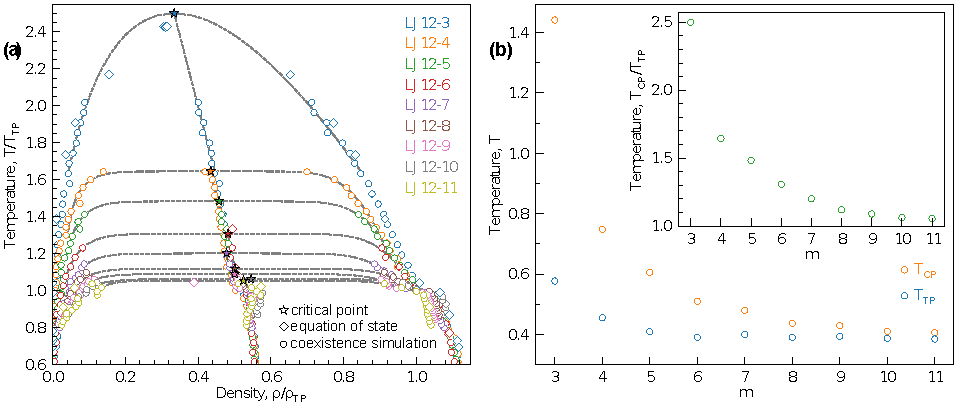
\includegraphics[width=\textwidth]{NMP-Figure4.pdf}
\caption{Влияние диапазона притяжения на область сосуществования жидкость-газ на фазовой диаграмме: (a) бинодали конденсат-газ для разных потенциалов LJ12-m; круги — точки бинодали и медианы (полученные методом фазовой идентификации), ромбы — точки, полученные из уравнения состояния, серые линии — аппроксимации бинодали, звездочками обозначены критические точки.
	(b) Зависимости тройной и критической температур от индекса притяжения m для взаимодействия LJ12-m, отношение $T_{CP}$/$T_{TP}$ показано на вставке.}
\label{nmp}
\end{center}
\end{figure}

Падение диапазона притяжения снижает критическую температуру, а также отношение между температурами критической и тройной точек, как показано на рисунке~\ref{nmp}(b) и соответствующей вставке. 
С увеличением $m$ (ближнее притяжение) двухфазная область сужается в сторону меньших плотностей, а отношение между критической и тройной температурами приближается к единице. 
Для LJ-взаимодействия ($m = 6$) полученная критическая температура $T_c=(0,51 . . . 0,52)$ (в зависимости от метода оценки) согласуется с предыдущими результатами $T_c = 0.515 \pm 0.002$  для LJ-потенциала.

В данном разделе был проведен обзор эволюции фазовых диаграмм и сценариев плавления двумерных систем частиц, взаимодействующих через обобщенный потенциал Леннарда-Джонса с разным диапазоном притяжения, в то время как ветвь отталкивания зафиксирована.
%какая ветвь? откуда? её не было, как и слов о фиксации. я нашла этот момент в статье, но только там эта ветвь упоминается ещё 3 раза до этого, а у тебя - ни одного. я оставила тебе перевод с нужной передачей смысла, но подумай, нужно ли оно вообще
Переход жидкость-газ изучается с помощью анализа уравнения состояния и метода фазовой идентификации.
Результаты, полученные двумя упомянутыми методами, хорошо согласуются друг с другом.
Плавление при высоких температурах (и высоких плотностях) в системе мягких сфер $1/r_{12}$ происходит согласно третьему сценарию. 
Однако при низких температурах плавления в системах с $m = 6$, $9$ и $11$ было выявлено изменение сценария плавления от третьего сценария к переходу первого порядка (без гексатической фазы).
Было обнаружено, что температура изменения сценариев смещается в сторону более низких температур с увеличением диапазона притяжения (что соответствует уменьшению $m$). 
Анализ случая $m = 9 (LJ12-9)$  показал, что для короткодействующего притяжения наблюдается третий сценарий плавления.

Однако на данный момент не существует теории, которая предсказывала бы поведение транспортных свойств и коллективных возбуждений в зависимости от дальнодействия притяжения.
В связи с этим формулируются следующие цели и задачи настоящей работы.

\section{Цели и задачи магистерской работы}

\textbf{Цель работы} -- установить связь дальнодействия притяжения потенциала взаимодействия и спектров возбуждений с транспортными свойствами жидкостей, а также влияние на скорость нуклеации.

\textbf{Задачи работы:}
\begin{enumerate}
    \item Расчет фазовых диаграмм для 2D и 3D систем частиц, взаимодействующих посредством обобщенного потенциала Леннарда--Джонса с различными степенями притяжения.
    \item Адаптация метода кластеризации данных DBSCAN для изучения молекулярных систем и его сравнение с другими методами.
    \item Расчет и анализ транспортных свойств и коллективных возбуждений на жидкостных бинодалях.
    \item Применение нового метода распознавания фаз для изучения скорости нуклеации в переохлажденных системах Леннарда-Джонса с различным дальнодействием притяжения.
\end{enumerate}


\newpage
\begin{center}
\textbf{\large ГЛАВА 2 \\ Модель плавления перегретых кристаллов}
\end{center}
\refstepcounter{chapter}
\addcontentsline{toc}{chapter}{ГЛАВА 2. Модель плавления перегретых кристаллов}


\section{Введение}

Плавление - один из наиболее изученных фазовых переходов, важных для атомных, молекулярных, коллоидных и белковых систем.
Однако в настоящее время не существует микроскопических экспериментально доступных критериев, которые можно было бы использовать для надежного отслеживания эволюции системы при переходе, дающих возможность  понять физику зародышеобразования при плавлении и эволюции фронта плавления.
Чтобы решить эту проблему, разработана теоретическая модель в рамках теории среднего поля с использованием нового локального параметра порядка (экспериментально измеримого) -- нормированного среднеквадратичного смещения между частицами в соседних ячейках Вороного.
Предложенная модель протестирована при помощи компьютерного моделирования, при различных режимах динамики частиц (броуновским и ньютоновским), и в результате обнаружено, что она обеспечивает превосходное описание эволюции системы при пересечении линии плавления.

Явление плавления широко распространено в природе и может быть обнаружено начиная, от атомных и молекулярных до белковых и коллоидных систем, и выходит далеко за рамки материаловедения, поэтому при формулировке критериев плавления в микроскопическом масштабе уделяется значительное внимание уже не менее 100 лет.
Один из наиболее широко используемых микроскопических подходов принадлежит Линдеману \cite{lindemann1910} и, в частности, его переосмысление Гилварри \cite{10.1103/physrev.102.308}: то, что сейчас известно как критерий Линдемана, утверждает, что плавление происходит, когда среднеквадратичное смещение атомов от их положения достигает определенной доли (обычно 0.1-0.15) межатомного расстояния.
Популярность критерия обусловлена его простотой и интуитивно понятной способом применения, но есть и существенные недостатки, включая низкую точность в прогнозировании температуры плавления и отсутствие явного учета жидкого состояния \cite{10.1098/rspa.1991.0068}.
Впоследствии, был введен ряд критериев, которые можно проследить до работы Гилварри \cite{10.1063/1.1426419}, в частности, с развитием современных экспериментальных и вычислительных методов, которые обеспечивают доступ к смещениям атомов.
Однако детали структурных изменений, особенно в отношении этих критериев, остаются неуловимыми, а ряд ключевых явлений, включая детали механизма зародышеобразования, кинетики фронта плавления и поведения системы вблизи точки плавления, остаются малоизученными.


\section{Материалы и методы}

\subsection{$\lambda^2$-Параметр: Локальная мера беспорядка}
\label{SSMF-AppA}

В работе~\cite{10.1021/acs.jpcc.7b09317}, для характеризации локальной разупорядоченности и идентификации конденсированных (жидких или твердых) фаз в конденсируемых системах был предложен подход, основанный на анализе ячеек Вороного -- элементарной площади (''объема''), занимаемой каждой частицей в системе.
В рамках подхода на первом этапе система разбивается на ячейки Вороного, чтобы вычислить следующий параметр:
\begin{equation}
\label{SSMF-eq1}
\sigma_{i} =\frac{1}{a_i N_{ni}}\sqrt{\sum_{j<k}^{N_{ni}}{(r_{ij}-r_{ik})^2}/2}, \quad r_{ij}=|\mathbf{r}_i-\mathbf{r}_j|,
\end{equation}
где $\mathbf{r}_i$ -- радиус-вектор $i$-ой частицы, $N_{ni}$ -- количество соседних ячеек, $a_i = \sqrt{S_i/\pi}$ -- характерный радиус, $S_i$ -- площадь ячейки Вороного.
На втором этапе для подавления сильных локальных тепловых флуктуаций проводится усреднение с соседними ячейками, которые имеют общую грань (сторона в 2D случае) с ячейкой частицы $i$ \cite{10.1021/acs.jpcc.7b09317}:
\begin{equation}
\label{SSMF-eq2}
\lambda_{i} = \frac{1}{N_{ni}+1}\left(\sigma_{i}+\sum_{j=1}^{N_{ni}}{\sigma_{j}}\right).
\end{equation}
В результате получается стандартное отклонение $\lambda_i^2$ расстояний между соседними частицами в \emph{физически малом объеме} в окрестности $i$-й частицы.
Важно отметить, что $\lambda_i^2$ одинаково хорошо применимо для характеризации как твердой, так и жидкой фаз системы, поскольку этот параметр связан с локальным беспорядком в физически малом объеме \cite{10.1021/acs.jpcc.7b09317}.
В кристаллах $\lambda^2$ связано с параметром Линдемана для соседних частиц \cite{10.1016/0375-9601(85)90617-6}, поскольку $\lambda^2 \propto \sigma_\|^2$, где $\sigma_\|^2$ - продольная компонента среднеквадратичного смещения ближайших частиц.


\subsection{Детали моделирования МД}
\label{SSMF-AppC}

Проведено МД-моделирование кристаллов в условиях ланжевеновской динамики.
В качестве характерного примера рассмотрена система частиц, взаимодействующих по обратному степенному закону (IPL18):
\begin{equation}
\label{SSMF-eq3}
\varphi(r) = \epsilon a \left(\frac{\sigma}{r}\right)^{18},
\end{equation}
где $\epsilon$ и $\sigma$ -- сила и характерный масштаб отталкивания соответственно,
а параметр $ a = 2.365 $ введен для удобства моделирования скачкообразного изменения диаметра частиц.
Использовалась нормированная температура $ T/ \epsilon \rightarrow T $, расстояние $ r/ \sigma \rightarrow r $, плотность частиц $\rho\sigma^3/m\rightarrow n$ и время $t\sqrt{\epsilon/m\sigma^2} \rightarrow t$ ($m$ -- масса частицы).

Для анализа плавления перегретого кристалла выполнено МД-моделирование системы, состоящей из $ N = 7.2 \times 10 ^ 4 $ частиц в $NVT$ ансамбле при $n=0.867$ и $T=1$.
В исходном состоянии частицы располагались в ГЦК решетке, ориентированной таким образом, чтобы плоскость (111) совпадала с горизонталью.
Размеры области моделирования в $ x $, $ y $ и $ z $ -направлениях были выбраны так, чтобы $ L_x / L_z \approx 20.4 $ и $ L_y / L_z \approx 21.3 $.
Временной шаг был выбран равным $ \Delta t = 7.4 \times 10 ^ {- 4} \sqrt {m \sigma ^ 2 / \epsilon} $. Расчеты методом молекулярной динамики проводились в открытом программном пакете LAMMPS.
Моделирование проводилось в 2 этапа: (i) система моделировалась на протяжении $ 10 ^ 5 $ временных шагов с $ a = 7.224 $ для достижения состояния равновесия; (ii) значение $a$ фиксировалось равным $ 2.365 $ и проводилось дополнительное моделирование на $ 4 \times 10 ^ 5 $ шагов для анализа плавления в кристалле.

\section{Результаты}
\subsection{Самосогласованная модель среднего поля эволюции $\lambda^2$ - поля}

Примеры кристаллических и жидких структур показаны на Рис.~\ref{SSMF-Figure1}(a) и \ref{SSMF-Figure1}(b) соответственно.
Белые точки -- это частицы, ячейки Вороного показаны сплошными серыми линиями, и окрашены в соответствии со значением параметра $\lambda^2$ -- нормированным среднеквадратичным смещением между частицами в соседних ячейках Вороного \cite{10.1021/acs.jpcc.7b09317}. %(см. раздел~\ref{SSMF-AppA}).
В кристаллах $\lambda^2$ связано с параметром Линдемана для соседних частиц \cite{10.1016/0375-9601(85)90617-6}.
Это обусловлено тем, что $\lambda^2\propto \sigma_ \| ^ 2 $, где $ \sigma_ \| ^ 2 $ является продольной составляющей среднеквадратичного смещения ближайших частиц.
Кроме того, $ \sigma_ \| ^ 2 $ играет важную роль в вычислении первого корреляционного пика в кристаллах \cite{10.1063/1.4869863, 10.1063/1.4926945, 10.1088/0953-8984/28/23/235401, 10.1039/c7sm02429k, 10.1063/1.5116176}.
После плавления кристаллическая решетка разрушается, но, несмотря на диффузию частиц, разбиение Вороного все еще применимо в жидкости.

В случае систем с отталкиванием, рост $\lambda^2$ обеспечивается (i) повышением температуры или (ii) уменьшением плотности.
В то время как первый механизм играет центральную роль в системах с мягким отталкиванием между частицами (например, в мягких кристаллах при низких температурах $\lambda^2\propto T $), последний является определяющим в системах типа твердых сфер (таких как коллоиды NIPAm), коллективная динамика которых определяется объемной долей частиц.
В обоих случаях $\lambda^2$ играет роль параметра порядка, и в этих терминах плавление представляет собой переход от состояний с малым $\lambda^2$ (кристалл) к состояниям с большим $\lambda^2$ (жидкость).

Чтобы получить самосогласованную модель эволюции $ \lambda^2$-поля,
необходимо рассмотреть слабо неоднородное пространственное поле $\lambda^2$.
Параметр $\lambda ^ 2$ неконсервативен, а следовательно его эволюция определяется нестационарным уравнением Гинзбурга-Ландау (или моделью Ланжевена) \cite{book.desai}:
\begin{equation}
\label{SSMF-eq4}
\frac{\partial \lambda^2}{\partial t} = -\Gamma \frac{\delta \mathcal{F}}{\delta \lambda^2} + \varepsilon^{1/2}\xi(t,\mathbf{r}),
\end{equation}
где $\Gamma$ -- обобщенная вязкость, $ \mathcal{F} $ -- функционал свободной энергии системы, $\langle \xi(t,\mathbf{r})\xi(t',\mathbf{r}')\rangle = \delta(t-t')\delta(\mathbf{r}-\mathbf{r}')$ и $\varepsilon = 2k_BT\Gamma$.
Последнее слагаемое в~\eqref{SSMF-eq2} описывает тепловые флуктуации поля $\lambda^2$.

\begin{figure}[!t]
\centering
 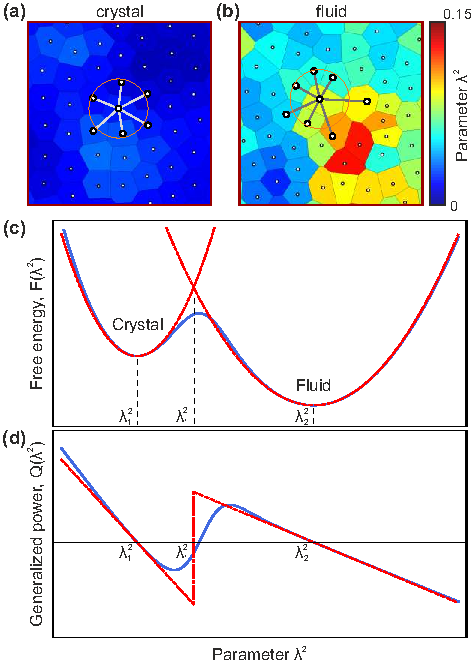
\includegraphics[width=100mm]{SSMF-Figure1.pdf}
 \caption{\textbf{Схематичное изображение к предлагаемой самосогласованной $\lambda^2$~-~модели:}
 (a) и (b) снимки системы в кристаллическом и жидком состоянии (взяты из МД моделирования).
  Ячейки Вороного раскрашены в соответствии со значениями параметра $ \lambda^2$.
  Панели (c) и (d) схематично иллюстрируют (синие линии) зависимость свободной энергии $ F (\lambda ^ 2) $ (в однородной системе) и обобщенную мощность $ Q (\lambda ^ 2) $, сопряженную с полем $\lambda^2$.
 Пунктирные красные линии иллюстрируют ступенчатое приближение \eqref{SSMF-eq5} и \eqref{SSMF-eq7}.
 }
\label{SSMF-Figure1}
\end{figure}


\begin{figure*}[!t]
\centering
 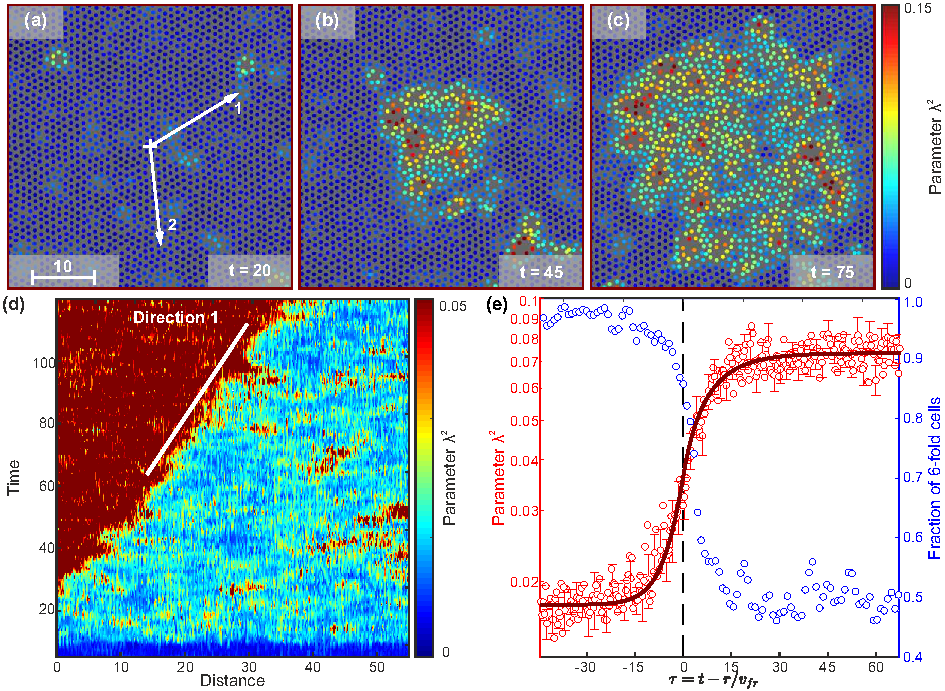
\includegraphics[width=\linewidth]{SSMF-Figure3.pdf}
 \caption{\textbf{Автомодельный $ \lambda^2$-профиль распространяющегося фронта плавления в перегретом кристалле, наблюдаемый при МД-моделировании:}
 (a) - (c) Последовательные снимки системы, где круги представляют собой частицы, окрашенные в соответствии со значением $\lambda^2$.
 (d) Эволюция поля $\lambda^2(r, t)$ в радиальном направлении (1), показанном на (a).
 (e) $\lambda^2(\tau)$ -- профиль распространяющегося фронта плавления при росте зародышей.
 Красные символы -- экспериментальные точки, красная сплошная линия -- теоретическая аппроксимация \eqref{SSMF-eq9}.
 Синие символы представляют собой долю ячеек Вороного с 6-ю соседями в плоскости анализа, а резкое падением, указывает на разрушение кристаллической структуры.}
\label{SSMF-Figure3}
\end{figure*}

Функционал свободной энергии $\mathcal{F}[\lambda^2] = \int{d\mathbf{r}\;F[\lambda^2]}$ в квадратичном приближении может быть представлен в виде:
\begin{equation}
\label{SSMF-eq5}
F[\lambda^2] = F_{\mathrm{1,2}}^{(0)}+\frac{1}{2}A_{1,2}\left(\lambda^2-\lambda_{1,2}^2\right)^2 + \frac{1}{2}\alpha_{1,2}\left(\nabla\lambda^2\right)^2,
\end{equation}
где $F_{1,2}^{(0)}$ -- энергия однородного состояния ($1$ или $2$), $A$ и $\alpha$ -- положительные коэффициенты разложения \cite{book.desai}, а индексы $ 1 $ и $ 2 $ соответствуют кристаллическому или жидкому состоянию при $\lambda^2 \lessgtr \lambda_\ast^2$ соответственно.
Параметр $\lambda_\ast^2 $ -- это порог, связанный с обобщенным критерием плавления типа Линдемана, и предполагается, что $ F_{\mathrm{1}} ^ {(0)}> F_{\mathrm{2}} ^ {(0)} $ для рассматриваемого случая.

При помощи уравнений~\eqref{SSMF-eq4} и \eqref{SSMF-eq5} можно получить:
\begin{equation}
\label{SSMF-eq6}
\frac{\partial \lambda^2}{\partial t} = \chi_{1,2} \nabla^2\lambda^2 + Q(\lambda^2) +  \varepsilon^{1/2}\xi(t,\mathbf{r}),
\end{equation}
где $ \chi_{1,2} = \alpha_{1,2} \Gamma $ -- характеризует диффузию $\lambda^2$,
а $ Q (\lambda ^ 2) $ -- обобщенный источник $ \lambda^2$-поля,
\begin{equation}
\label{SSMF-eq7}
Q(\lambda^2) =
\left\{
  \begin{array}{ll}
   -\gamma_{1}\left(\lambda^2-\lambda_{1}^2\right), & \lambda^2  < \lambda_\ast^2;\\
   -\gamma_{2}\left(\lambda^2-\lambda_{2}^2\right), & \lambda^2 > \lambda_\ast^2,\\
  \end{array}
\right.
\end{equation}
где $\gamma_{1,2} = \Gamma A_{1,2}$.
Уравнение \eqref{SSMF-eq6} демонстрирует аналогию с эволюцией температуры в химически реактивных средах \cite{10.1088/0004-637x/805/1/59} и совпадает с уравнением для кинетической температуры, которое исследовалось в работах~\cite{10.1103/physreve.96.043201, 10.1103/physreve.97.043206, 10.1103/physreve.100.023203} при анализе распространяющихся фронтов неравновесного плавления в однослойных пылевых плазменных кристаллах.

Энергия \eqref{SSMF-eq5} для однородного случая и соответствующая обобщенная мощность $ Q (\lambda ^ 2) $ показаны на Рис.~\ref{SSMF-Figure1}(с) и \ref{SSMF-Figure1}(d).
Как видно на Рис.~\ref{SSMF-Figure1}(d), система может существовать долгое время в окрестности устойчивых состояний с $\lambda^2= \lambda_{1,2} ^ 2 $, тогда как пороговое значение $\lambda^2=\lambda_\ast^2$ соответствует неустойчивой точке.
Ниже будет показано, что решение уравнения~\eqref{SSMF-eq6} объясняет два важных явления, изучаемых в настоящем исследовании:
(i) распространение автомодельных фронтов плавления в перегретых кристаллах, образованных частицами, движущимися в броуновском или ньютоновском динамическом режиме, и (ii) бифуркационное поведение различных $\lambda^2$ -флуктуаций (зародышей плавления) в перегретом кристалле.

Если пренебречь влиянием теплового шума и полагать кривизну фронта плавления незначительной при его распространении, то это означает, что $ \epsilon \simeq 0 $ и в уравнении~\eqref{SSMF-eq6} можно записать $ \nabla ^ 2 = \partial ^ 2 / \partial r ^ 2 $.
В этом случае, самоподобный профиль (бегущей волны плавления) описывается функцией $\lambda^2(t-r/v_\mathrm{fr})\equiv \lambda^2(\tau)$ (где $v_\mathrm{fr}$ -- скорость фронта), которая подчиняется уравнению:
\begin{equation}
\label{SSMF-eq8}
\frac{\chi_{1,2}}{v_{\mathrm{fr}}^2} \frac{d^2 \lambda^2}{d\tau^2} -\frac{d \lambda^2}{d \tau} -\gamma_{1,2}(\lambda^2-\lambda_{1,2}^2) =0,
\end{equation}
учитывая, что $\lambda^2(\tau) $ и его производная $ d\lambda^2/ d \tau $ должны быть непрерывными в точке $ \tau = 0 $, где $\lambda^2=\lambda_\ast^2$.
Полученное уравнение идентично уравнению, которое возникает в задаче неравновесного плавления в комплексных (пылевых) плазменных кристаллах, а следовательно, решение уравнения~\eqref{SSMF-eq8} аналогично \cite{10.1103/physreve.96.043201, 10.1103/physreve.100.023203}:
\begin{equation}
\label{SSMF-eq9}
\frac{\lambda^2(\tau)-\lambda^2_1}{\lambda^2_\ast-\lambda^2_1}=
\left\{
  \begin{array}{ll}
    e^{p_1 \tau}, & \tau < 0;\\
   1+\left(1-e^{-p_2\tau}\right)p_1/p_2 , & \tau > 0,\\
  \end{array}
\right. \\
\end{equation}
где $ p_{1,2} = \left(\sqrt {1 + 4 \gamma_{1,2} \chi_{1,2} / v_\mathrm{fr} ^ 2} \pm 1 \right) v_\mathrm{fr} ^ 2/2 \chi_{1,2} $ -- показатели в экспоненциальных ветвях решения до и после фронта плавления.
В пределе $\tau \gg 1$, $\lambda^2(\tau) \rightarrow \lambda_2^2$, откуда следует, что
$\left(\lambda_2^2-\lambda^2_1\right)/\left(\lambda^2_\ast-\lambda^2_1\right) = (1+p_1/p_2)$.
Скорость фронта плавления и показатели $p_{1,2} $ (неизвестные \emph{априори}) сложным образом определяются диффузией $\lambda^2$, спецификой межчастичных взаимодействий и различием химических потенциалов на границе жидкость-твердое тело~\cite{10.1038/ncomms7942}.


\subsection{Прямое наблюдение автомодельного профиля стационарных фронтов плавления в МД симуляции}
\label{SSMF-Results-MD}

Распространение фронтов плавления -- медленный процесс по сравнению с характерным временем движения отдельных частиц.
Это означает, что описание в терминах медленно флуктуирующего $\lambda^2$-поля должно быть применимым как в коллоидах, демонстрирующих броуновский режим движения отдельных частиц, так и в системах с ланжевеновской динамикой.
Чтобы подтвердить, что все ключевые особенности, наблюдаемые в случае коллоидных систем, присутствуют и в атомарных кристаллах было выполнено моделирование аналогичного процесса методом МД с термостатом Ланжевена и слабым затуханием.
При параметрах выполненного МД-моделирования плотность системы при плавлении и кристаллизации (в безразмерных единицах) составляет $ n_m = 0,93 $ и $ n_f = 0,88 $, соответственно~\cite{10.1080/00268979500100911}.
Следовательно, ступенчатое изменение диаметра частиц в проведенных расчетах можно оценить как $ (n_f / n) ^ {1/3} -1 \simeq 0.5 \% $ ($ n = 0.867 $), это позволяет вычислить падение эффективной объемной доли частиц относительно ее значения, соответствующего плавлению, как
$\Delta \phi  \simeq (n_m/n)^{1/3}-1\simeq 2.4\%$.
Полученное значение близко к режиму промежуточного перегрева, обсуждаемому в работе~\cite{10.1038/ncomms7942}.


Результаты проведенного МД-моделирования автомодельных фронтов плавления в перегретом кристалле частиц с IPL18 взаимодействием представлены на Рис.~\ref{SSMF-Figure3}.
Полученные значения $\lambda^2$ в кристаллическом, жидком и пороговом состояниях равны $\lambda_1^2 \simeq 0.01$, $\lambda_2^2 \simeq 0.07$, и $\lambda_\ast^2 \simeq 0.035$, соответственно.
Значения $\lambda_\ast^2$, полученные в МД моделированиях хорошо согласуются с критерием Линдемана для ближайших соседей \cite{10.1016/0375-9601(85)90617-6}.


\section{Заключение главы}

Поведение поля $\lambda^2$ было проанализировано с использованием нестационарного уравнения Гинзбурга-Ландау с тепловым шумом и источниками.
Показано, что разработанная модель демонстрирует существенно нелинейное поведение, в то время как слагаемые в уравнениях имеют ясный физический смысл в контексте анализа плавления кристаллов.
Кроме того, будучи по своей сути микроскопической, предложенная модель позволяет с высокой степенью детализации изучать зародышеобразование в различных режимах перегрева (в зависимости от величины теплового шума) и эволюцию реалистичных жидких зародышей, которые могут принимать самые разные сложные формы.


Процесс зародышеобразования в перегретых кристаллах, кинетика образования и роста жидких зародышей и структура устойчивых фронтов плавления представляют собой центральные проблемы для понимания плавления кристаллов.
Представленные результаты являются существенным шагом вперед, предоставляя простой и эффективный инструмент для изучения процессов зародышеобразования и плавления в перегретых кристаллах различной природы.



\newpage
\begin{center}
\textbf{\large ГЛАВА 3 \\ Диффузия на жидких бинодальях: влияние дальнодействия силы притяжения}
\end{center}
\refstepcounter{chapter}

\addcontentsline{toc}{chapter}{ГЛАВА 3. Диффузия на жидких бинодальях: влияние дальнодействия силы притяжения}

В этой работе мы используем моделирование молекулярной динамики для расчета фазовых диаграмм обобщенных систем Леннарда-Джонса с различными показателями притяжения. Оценены коэффициенты диффузии и подвижности (обратной диффузии) и проанализированы спектры коллективного возбуждения на жидких бинодалиях. Отмечено, что зависимость коэффициента подвижности от температуры является линейной в широком диапазоне температур, а ее наклон увеличивается с увеличением показателя притяжения. В начале нелинейной зависимости подвижности от температуры дисперсионные соотношения коллективных возбуждений жидкости обнаруживают переход от колебательного к монотонному ходу.

\section{Введение}
\label{MACR-SecIntroduction}

Диффузия играет важную роль в различных процессах переноса массы, начиная от науки и техники и заканчивая живой природой.
Он играет решающую роль в биологических процессах~\cite{10.1016/j.bbagen.2013.09.037, 10.1038/s41598-018-22643-9}, а также в механизмах и кинетике химических реакций. Знание механизмов диффузии позволит добиться значительного прогресса в новых биотехнологиях и медицине, решить важные проблемы химической и фармакологической промышленности и не только~\cite{10.1002/3527602836}.

Процесс диффузии очень хорошо изучен в газах и твердых телах. Например, очень подробное знание процесса диффузии достигается в кристаллических системах~\cite{10.1016/0079-6816(95)00039-2} из-за его практической важности в металлургии для легирования~\cite{10.1016/s0924-0136(96)02826-9, 10.1016/j.actamat.2015.10.010, 10.1134/s1063783411110308} и эксплуатации полупроводниковой электроники~\cite{10.1103/physrevlett.84.4220, 10.1016/j.physrep.2009.10.003}.

Наше понимание процесса диффузии в жидкостях остается довольно ограниченным и фрагментарным, хотя за прошедшие годы был достигнут некоторый прогресс~\cite{FrenkelBook,HansenBook,GrootBook,MarchBook}.
Существуют приближенные скейлинги и соотношения, которые могут с разной степенью точности описывать диффузию в разных системах. Пожалуй, простейшей оценкой температурной зависимости коэффициента диффузии в жидкости является закон Аррениуса~\cite{10.1126/science.278.5336.257}. Однако пренебрежение динамической вязкостью и другими особенностями реального потенциала взаимодействия делает его непригодным для точного определения коэффициента диффузии в широком диапазоне температур. Среди других полезных соотношений, касающихся диффузии в жидкостях, можно упомянуть избыточное энтропийное масштабирование коэффициентов переноса~\cite{10.1103/physreva.15.2545, 10.1038/381137a0, 10.1063/1.5055064}, их скейлинги температуры замерзания и плотности~\cite{10.1103/physreve.62.7524, 10.1063/1.5022058, 10.1063/1.5044703, 10.1103/physreve.103.042122}, а также соотношение Стокс-Эйнштейна между коэффициентами вязкости диффузии и сдвига~\cite{10.1063/1.446338, 10.1002/BBPC.19900940313, 10.1103/physreve.95.052122, 10.1063/1.5080662, 10.1080/00268976.2019.1643045}. Существуют методы, позволяющие достаточно точно прогнозировать диффузию в конкретных системах, в том числе в широком интервале температур, вплоть до критической точки и в закритической области~\cite{10.1063/1.1607953, 10.1016/j.camwa.2019.11.012, 10.1063/1.441097}. Доступны обширные результаты численного моделирования~\cite{10.1063/1.1786579, 10.1016/j.fluid.2011.03.002}. В настоящее время применяются методы машинного обучения~\cite{10.1063/5.0011512}.
Однако остаются открытыми такие важные вопросы, как влияние потенциала взаимодействия между частицами на температурную зависимость коэффициента диффузии и насколько важны корреляции между спектрами возбуждения частиц и транспортными свойствами.

В этой статье, используя метод молекулярной динамики (МД), мы моделируем обобщенные системы Леннарда-Джонса с различными показателями притяжения. Рассчитаны температурные зависимости подвижности частиц (коэффициента обратной диффузии) на бинодали жидкости. Нашей основной целью является установление связи между диффузией, размахом межчастичного притяжения и свойствами коллективных возбуждений в простых жидкостях.

\subsection{Методы}
\label{MACR-SecMethods}

Мы анализируем транспортные свойства и их связь с коллективными модами на жидких бинодальях.
для систем, взаимодействующих через обобщенный потенциал Леннарда-Джонса (LJ$n$-$m$):
\begin{equation}
U_{n-m}(r)=4 \varepsilon\left[\left(\frac{\sigma}{r}\right)^{n}-\left(\frac{\sigma}{r}\right)^{m}\right]
\label{MACR-eq1}
\end{equation}
где $\epsilon$ и $\sigma$ — характерные масштабы энергии и длины соответственно. На протяжении всей статьи используются приведенные единицы измерения температуры $ T/ \epsilon \rightarrow T $, расстояния $ r/ \sigma \rightarrow r $ и плотности $ \rho \sigma ^ 3 \rightarrow n$.


Мы рассмотрели потенциалы LJ$12$-$4$, LJ$12$-$5$, LJ$12$-$6$ и LJ$16$-$6$. Мы также смоделировали этан~\cite{10.1021/acs.jced.6b01036}, чтобы сравнить полученные результаты для LJ$n$-$m$ с результатами для системы, в которой взаимодействия не являются сферически-симметричными.
В выбранной модели молекула этана рассматривается как пара жестко связанных радикалов CH$_3$, взаимодействующих с радикалами других молекул через потенциал~\cite{10.1021/acs.jced.6b01036}:
\begin{equation}
U_{\rm {ethane}}(r) = \tilde \varepsilon\left[\left(\frac{\sigma}{r}\right)^{16}-\left(\frac{\sigma}{r}\right)^{6}\right],
\label{MACR-eq2}
\end{equation}
где $\tilde\varepsilon = 0,69396$ ккал/моль и $\sigma = 3,783$\AA.

Все МД-симуляции были выполнены в ансамбле NVT (N, V и T - количество частиц, объем системы и температура соответственно) с периодическими граничными условиями с использованием пакета моделирования LAMMPS~\cite{10.1006/jcph.1995.1039} .
На первом этапе были рассчитаны линии бинодали по ссылкам~\cite{10.1021/jp806127j, 10.1021/jp1117213}.
Исходное состояние системы формировалось в два этапа: (i) кубический ящик моделирования заполнялся равновесным кристаллом (в нашем случае ГЦК) из $N$ частиц с плотностью, соответствующей близкому к нулю давлению; (ii) окно моделирования было расширено в направлении осей $x$ так, чтобы окончательная средняя плотность системы $\rho_a$ стала равной значениям, указанным в таблице~\ref{MACR-Table1}.
Результирующее начальное состояние показано на рис.~\ref{MACR-Figure1}(а).
Затем температура системы линейно увеличивалась от $T_{start}$ до $T_{stop}$ в течение $n_{step}$ шагов моделирования с временным шагом $\Delta t$.
Конденсированная фаза в какой-то момент начинает испаряться, образуя сосуществование газа и конденсата, если температура ниже критической, как показано на рис.~\ref{MACR-Figure1}(b).
Принципиально то, что полученное таким образом состояние системы почти всегда имеет границы фаз, ортогональные оси $x$.
В результате плотности $\rho_g$ и $\rho_c$ газовой и конденсированной фаз соответственно могут быть рассчитаны путем подгонки профиля плотности $\rho(x)$ выражением~\cite{10.1021/jp806127j, 10.1021/jp1117213}:

\begin{equation}
    \rho(x)=\frac{\rho_{l}+\rho_{g}}{2}-\frac{\rho_{l}-\rho_{g}}{2} \tanh \left(\frac{|x|-L}{\delta}\right),
    \label{MACR-eq3}
\end{equation}
где $L$ — половина площади, занимаемой жидкой фазой, а $\delta$ — характерная ширина границы раздела.
Пример профиля плотности системы и его аппроксимация уравнением~\eqref{MACR-eq3} показаны на рис.~\ref{MACR-Figure1}(c) гистограммой и красной линией соответственно.
Параметры моделирования для рассмотренных моделей сведены в табл.~\ref{MACR-Table1}.

% \renewcommand{\arraystretch}{1.25}
% \begin{table}[h!]
%     \centering{
%     \begin{tabular}{>{\centering}p{1.3cm}|>{\centering}p{1.1cm}|>{\centering}p{1.0cm}|>{\centering}p{1.0cm}|>{\centering}p{1.0cm}|>{\centering}p{1.0cm}|>{\centering}p{1.0cm}>{\centering}p{0cm}}
%         Potential & $\rho_a$ & $r_c$ & $T_{\rm start}$ & $T_{\rm stop}$ & $n_{step}$& $\Delta t$ &\\  \hline
%         \multicolumn{8}{c}{Values in dimensionless units:} \\\hline
%         LJ12-4 & 0.25 & 15.0 & 1.0 & 5.5 & \multirow{4}*{$3 \times 10^6$}  & \multirow{4}*{$5 \times 10 ^ {- 4}$} &\\
%         LJ12-5 & 0.25 & 10.0 & 0.8 & 2.4 & & &\\
%         LJ12-6 & 0.35 & 8.0 & 0.5 & 1.4 &  & &\\
%         LJ16-6 & 0.31 & 8.0 & 0.8 & 1.6 &  & &\\ \hline
%         \multicolumn{8}{c}{Values in SI units:} \\\hline
%         Ethane & $0.22\mathrm{\frac{g}{cm^3}}$     & $25\mathrm{\AA}$ & $80\,\mathrm{K}$ & $320\,\mathrm{K}$ & $2 \times 10^6$ & $2\,\mathrm{fs}$ &
%     \end{tabular}
%     }
%     \caption{\textcolor{red}{Parameters used in MD simulations for the bimodal calculations: where $\rho$ is the average density of the system, $r_c$ is the cutoff radius, $T_{start}$ and $T_{stop}$ are the initial and final temperatures of the simulation, respectively, $n_{step}$ is the number of simulation steps, and $\Delta t$ is the timestep.
% }}
%     \label{MACR-Table1}
% \end{table}

\begin{table}[]
\centering
\begin{tabular}{|lllllcl|}
\hline
\multicolumn{1}{|l|}{Potential} & \multicolumn{1}{l|}{$\rho_a$} & \multicolumn{1}{l|}{$r_c$} & \multicolumn{1}{l|}{$T_{start}$} & \multicolumn{1}{l|}{$T_{stop}$} & \multicolumn{1}{l|}{$n_{step}$}                       & $\Delta t$                          \\ \hline
\multicolumn{7}{|c|}{Значения в безразмерных единицах:}                                                                                                                                                                                                         \\ \hline
\multicolumn{1}{|l|}{LJ12-4}    & \multicolumn{1}{l|}{0.25}     & \multicolumn{1}{l|}{15.0}  & \multicolumn{1}{l|}{1.0}         & \multicolumn{1}{l|}{5.5}        & \multicolumn{1}{c|}{\multirow{4}{*}{$3 \times 10^6$}} & \multirow{4}{*}{$5 \times 10^{-4}$} \\ \cline{1-5}
\multicolumn{1}{|l|}{LJ12-5}    & \multicolumn{1}{l|}{0.25}     & \multicolumn{1}{l|}{10.0}  & \multicolumn{1}{l|}{0.8}         & \multicolumn{1}{l|}{2.4}        & \multicolumn{1}{c|}{}                                 &                                     \\ \cline{1-5}
\multicolumn{1}{|l|}{LJ12-6}    & \multicolumn{1}{l|}{0.35}     & \multicolumn{1}{l|}{8.0}   & \multicolumn{1}{l|}{0.5}         & \multicolumn{1}{l|}{1.4}        & \multicolumn{1}{c|}{}                                 &                                     \\ \cline{1-5}
\multicolumn{1}{|l|}{LJ16-6}    & \multicolumn{1}{l|}{0.31}     & \multicolumn{1}{l|}{8.0}   & \multicolumn{1}{l|}{0.8}         & \multicolumn{1}{l|}{1.6}        & \multicolumn{1}{c|}{}                                 &                                     \\ \hline
\multicolumn{7}{|c|}{Единицы измерения СИ:}                                                                                                                                                                                                                     \\ \hline
\multicolumn{1}{|l|}{Ethane}    & \multicolumn{1}{l|}{$0.22\mathrm{\frac{g}{cm^3}}$}     & \multicolumn{1}{l|}{$25\text{\AA}$}    & \multicolumn{1}{l|}{$80\,\mathrm{K}$}          & \multicolumn{1}{l|}{$320\,\mathrm{K}$}        & \multicolumn{1}{l|}{$2 \times 10^6$}                  & $2\,\mathrm{\text{фс}}$                                   \\ \hline
\end{tabular}
\caption{Параметры, используемые в МД-моделировании для бимодальных расчетов: где $\rho$ — средняя плотность системы, $r_c$ — радиус отсечки, $T_{start}$ и $T_{stop}$ — начальная и конечная температуры. моделирования, соответственно, $n_{step}$ — количество шагов моделирования, а $\Delta t$ — временной шаг.}
\label{MACR-Table1}
\end{table}


\begin{figure}[!t]
\centering
 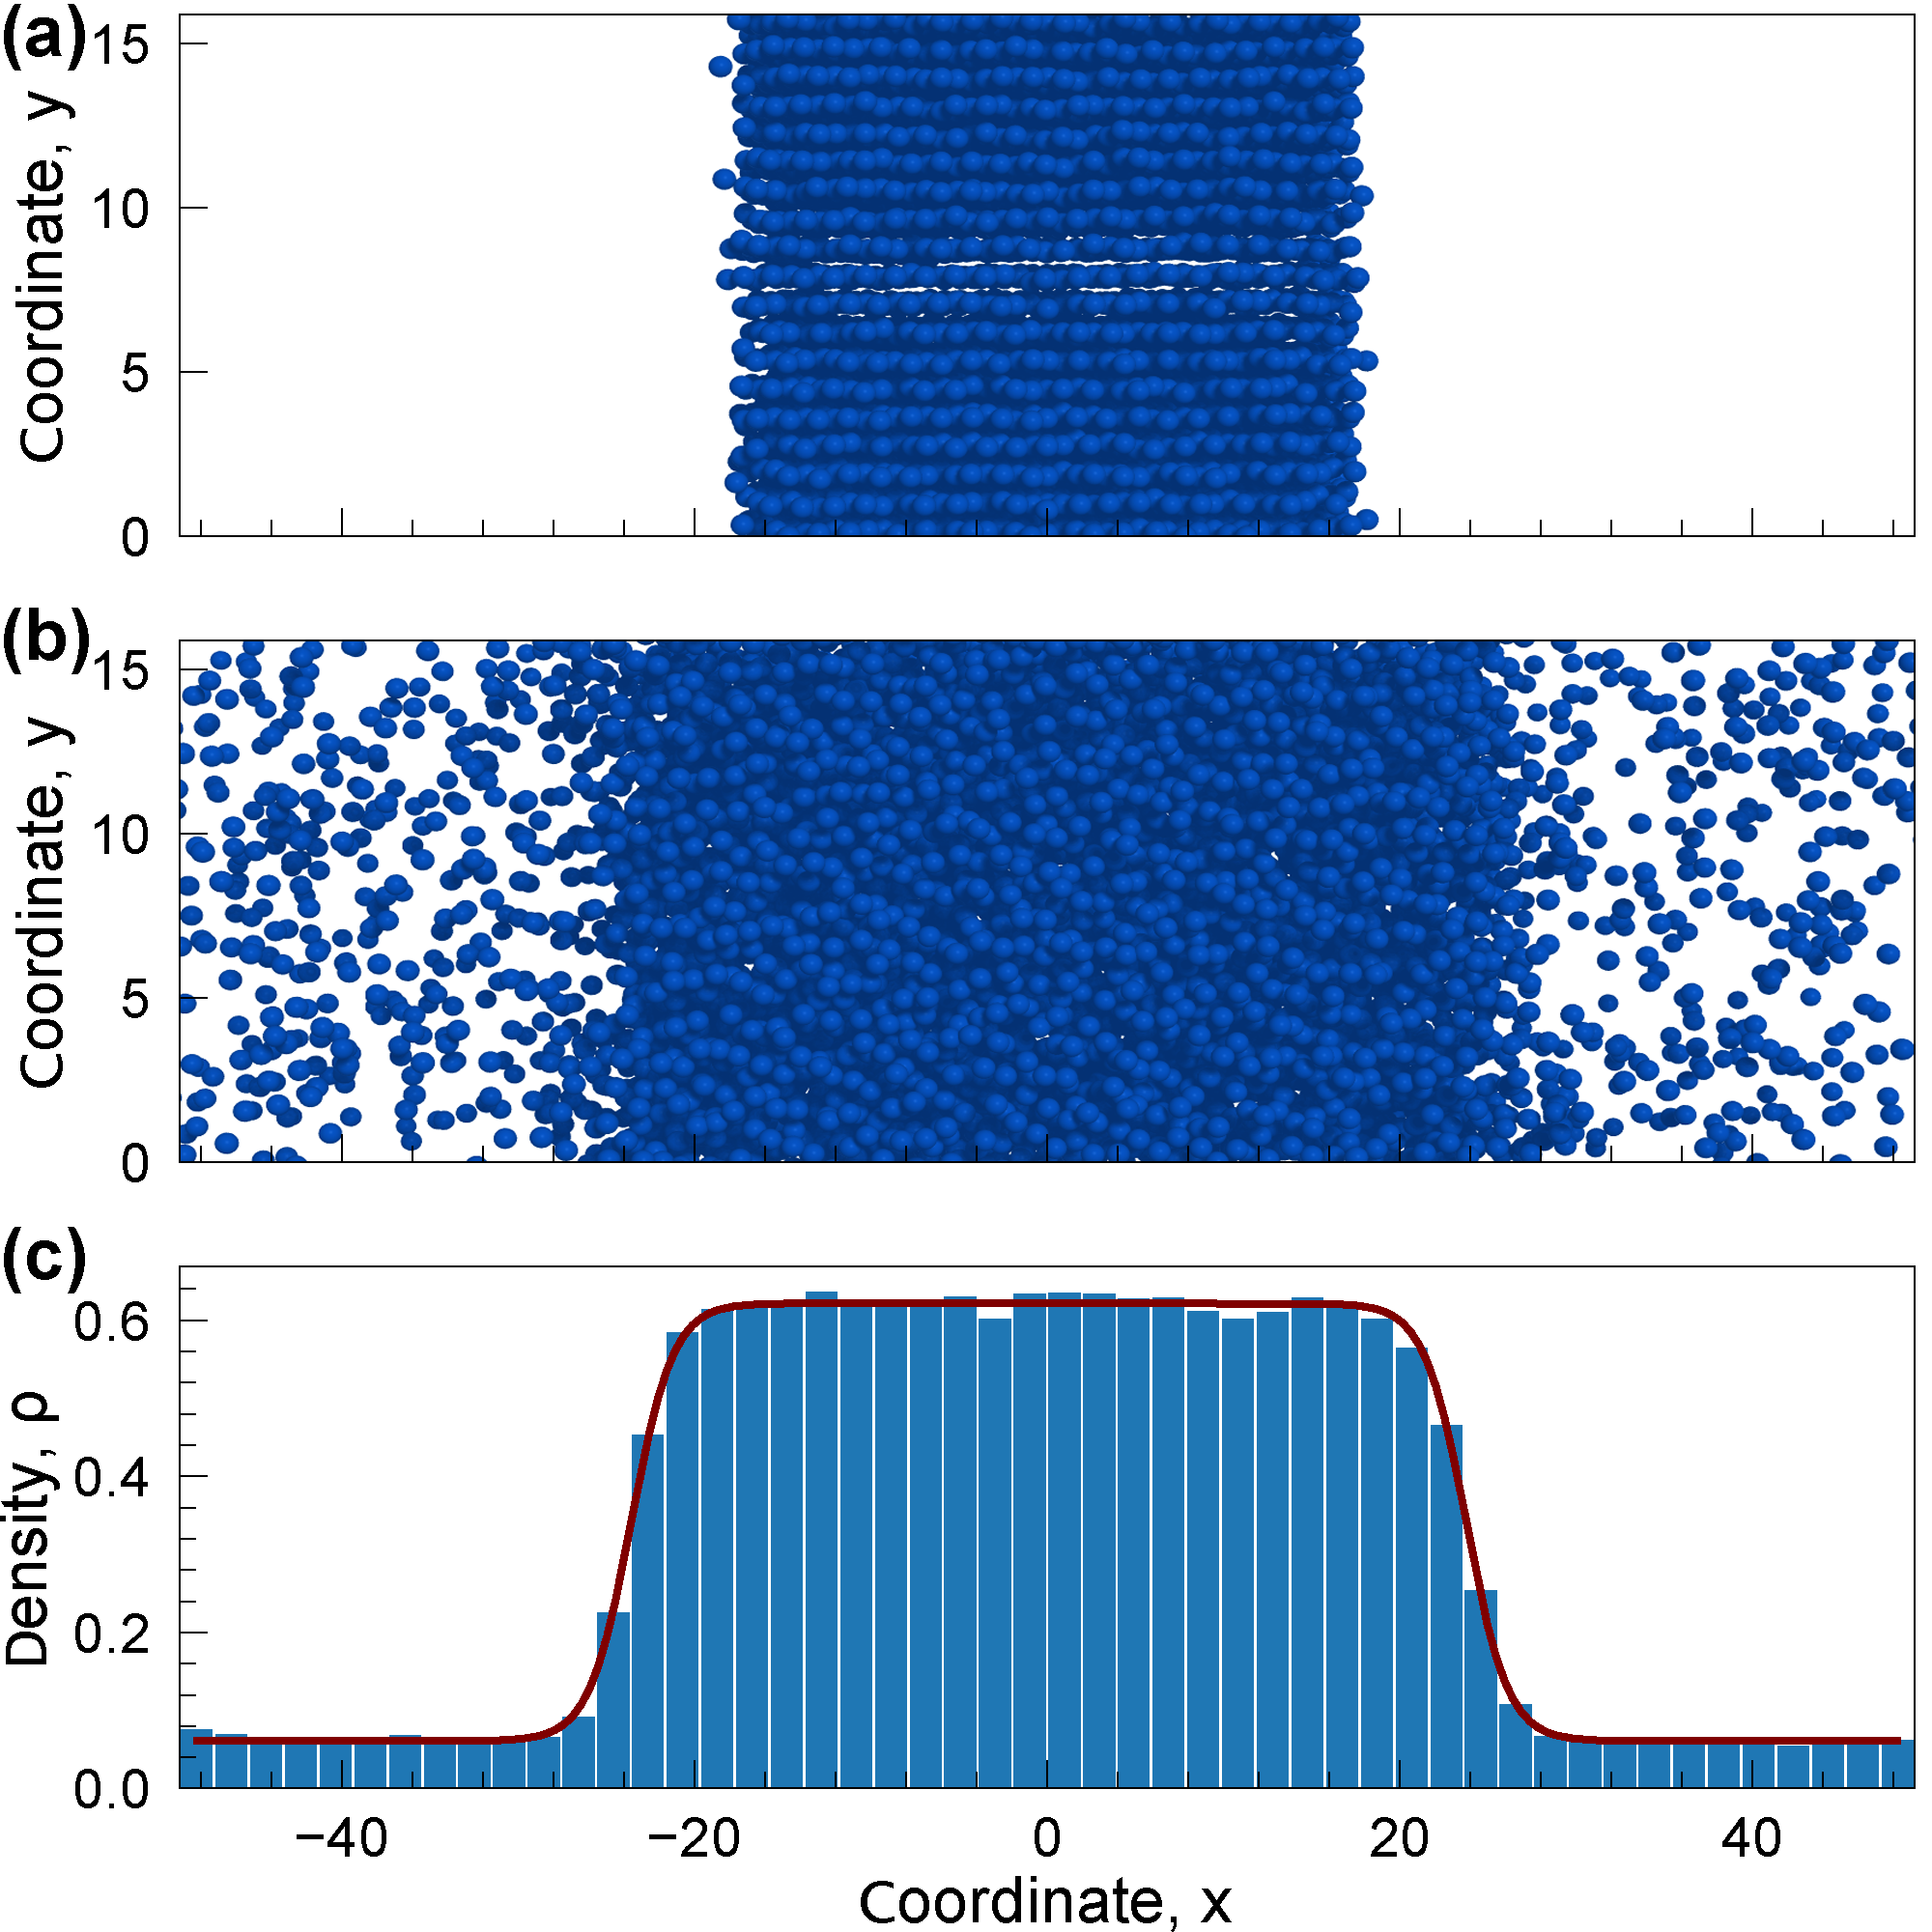
\includegraphics[width=85mm]{MACR-Figure1.png}
 \caption{(a) Система частиц для расчета фазовой диаграммы. Система частиц с потенциалом взаимодействия LJ12-6 при температуре $T=1.13$ в виде плоского слоя.
   (b) Профиль плотности системы вдоль оси $x$. Область с высокой плотностью представляет собой конденсат, с низкой - газ. Темно-красная линия представляет собой аппроксимацию профиля плотности уравнением~\eqref{MACR-eq3}.}
\label{MACR-Figure1}
\end{figure}


\begin{figure}[!t]
\centering
 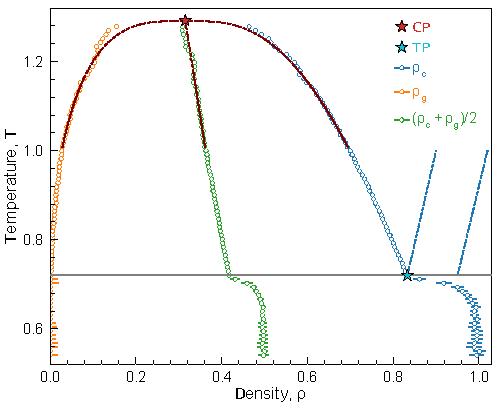
\includegraphics[width=85mm]{MACR-Figure2.pdf}
 \caption{Фазовая диаграмма системы LJ12-6.
  Оранжевые и синие символы — плотности газа и конденсата, полученные путем подгонки данных МД по уравнению~\eqref{MACR-eq3}.
  Зеленые символы — это медиана $\rho_m=(\rho_g+\rho_c)/2$.
  Сплошная красная линия соответствует уравнению~\eqref{MACR-eq4}.
  Тройные и критические точки обозначены синими и красными звездочками соответственно.
 }
\label{MACR-Figure2}
\end{figure}

Вблизи критической температуры расчет плотности газа и жидкости становится затруднительным из-за усиленных флуктуаций плотности.
Однако положение критической точки на фазовой диаграмме можно вычислить, аппроксимируя жидкостную и газообразную бинодальные ветви вблизи критической точки выражением:
\begin{equation}
    \rho_{l}-\rho_{g} \simeq A \tau^{\beta}, \quad \rho_{l}+\rho_{g} \simeq a \tau+2 \rho_{\mathrm{CP}},
\label{MACR-eq4}
\end{equation}

где $\tau=T_{\mathrm{CP}}-T$, $T_{\mathrm{CP}}$ и $\rho_{\mathrm{CP}}$ - температура и плотность в критической точке, $ \beta$ — критический индекс, $A$ и $a$ — свободные параметры.
Критический индекс $\beta$ зависит от класса универсальности системы, который определяется механизмами межчастичных взаимодействий~\cite{10.1103/physrevlett.89.025703}.
В трех пространственных измерениях критический индекс $\beta_c = 0,5$ для потенциала LJ$12-4$, тогда как $\beta_c = 0,325$ для LJ$12$-$5$, LJ$12$-$6$, LJ$16$-$6$ и этан, согласно предыдущим результатам~\cite{10.1021/acs.jced.6b01036,10.1021/jp9072137,10.1103/physrevlett.89.025703}.

Пример полученных бинодалей для LJ12-6 и их околокритическая аппроксимация уравнением~\eqref{MACR-eq4} показаны на рис.~\ref{MACR-Рисунок 2}.
Обратите внимание, что на конденсированной бинодали имеется явный излом (см. рис.~\ref{MACR-Рисунок 2}), который указывает на падение плотности при плавлении и соответствует положению тройной точки.
Полученные значения $A$ и $a$ аппроксимационного уравнения~\eqref{MACR-eq4}, а также плотности и температуры критических и тройных точек для рассматриваемых систем сведены в табл.~\ref{MACR-Table2}.

\begin{figure}[!t]
\centering
 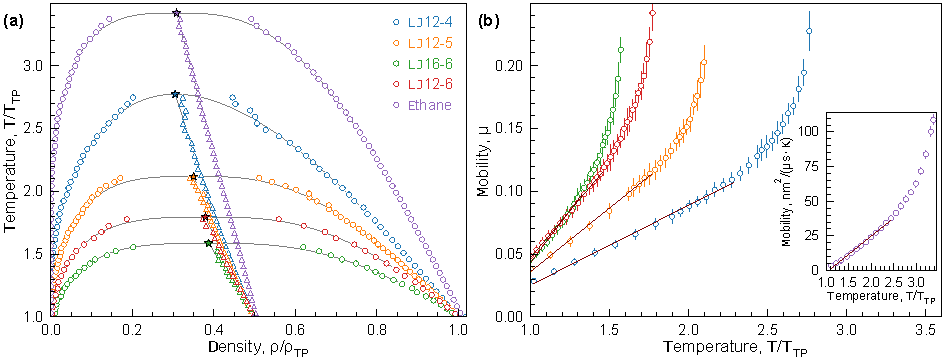
\includegraphics[width=170mm]{MACR-Figure3.pdf}
 \caption{(а) Фазовые диаграммы рассматриваемых систем. Фазовые диаграммы рассчитывались методом двухфазного моделирования, описанным в разделе~\ref{MACR-SecMethods}. Цветные точки обозначают рассчитанные бинодали, треугольники обозначают срединные точки. Сплошные серые кривые показывают диапазон температур, используемый для аппроксимации и определения параметров в уравнении ~\eqref{MACR-eq4}. Штриховые серые кривые соответствуют экстраполированным биноидам. (б) Температурная зависимость подвижности частиц. Подвижность частиц была рассчитана на жидких бинодальях с использованием метода, описанного в разделе~\ref{MACR-SecMethods}. Точки, соответствующие экстраполированным бинодалим, отмечены серым цветом. Прямые линии соответствуют линейной аппроксимации подвижности. На вставке показана расчетная подвижность метана.}
\label{MACR-Figure3}
\end{figure}

Далее для расчета подвижности на конденсированной бинодали моделировались системы с плотностью и температурой, взятыми из полученных фазовых диаграмм.
Для обобщенных леннард-джонсовских систем с $N = 4,0 \times 10 ^ 3$ моделировались шаги по времени $1,5 \times 10 ^ 5$. Для этана мы использовали $N = 1,065 \times 10 ^ 4 $ молекул и проводили моделирование с временными шагами $ 7,0 \times 10 ^ 5 $. Для релаксации системы использовались первые шаги по времени $ 5,0 \times 10 ^ 4 $ для обобщенных LJ-систем и шаги $ 5,0 \times 10 ^ 5 $ для этана. Остальные параметры были такими же, как и при расчете фазовых диаграмм.

Коэффициент самодиффузии $D$ определялся по среднеквадратичному отклонению частиц:
\begin{equation}
    \sigma^2(t) = \sum\limits_{\alpha = 1}^{N} (r_{\alpha}(t) - r_{\alpha}(0))^2 / N, \quad \sigma^2(t) = 6Dt,
    \label{MACR-eq5}
\end{equation}
где $\sigma$ — среднеквадратичное отклонение, а $t$ — время. Подвижность $\mu$ связана с коэффициентом диффузии соотношением Эйнштейна
\begin{equation}
    \mu = \frac{D}{T},
    \label{MACR-eq6}
\end{equation}
где $T$ — температура системы.

Наконец, спектры возбуждения были получены с использованием обработки тока скорости~\cite{10.1063/1.5050708}:
\begin{equation}
    C_{L, T}(\mathbf{q}, \omega)=\int dt e^{i \omega t} \text{Re} \left\langle\mathbf{j}_{L, T}(\mathbf{q}, t) \mathbf{j}_{L, T}(-\mathbf{q}, 0)\right\rangle,
    \label{MACR-eq7}
\end{equation}
где ${\bf k}$ и $\omega$ — волновой вектор и частота,
$\mathbf{j}_{L}=\mathbf{q}(\mathbf{j} \cdot \mathbf{q} ) / q^{2}$ и $\mathbf{j}_{T}=(\mathbf{j \cdot e_{\perp})e_{\perp}}$ — продольная ($L$) и поперечная ($T$) компоненты тока частиц,\\
$\mathbf{j}(\mathbf{q}, t)=N^{-1} \sum_{s} \mathbf{v}_{s}(t) \ exp \left(i \mathbf{q} \mathbf{r}_{s}(t)\right)$ и $\mathbf{v}_{s}(t)=\dot{\mathbf{r} }_{s}(t)$ — скорость $s$-й частицы.
Суммирование ведется по всем $N$ частицам в системе. Усреднение по каноническому ансамблю обозначается $\langle\cdots\rangle$. Анализ $C_{L, T}(\mathbf{q}, \omega)$ проводился по методикам, описанным в~\cite{10.1038/s41598-019-46979-y}, что позволило получить дисперсионные соотношения продольной и поперечной мод.

МД-моделирование для расчета спектров возбуждения отличается от моделирования для подвижности только длительностью временного шага. Для LJ$12$-$4$ и LJ$16$-$6$ шаг по времени был выбран как $\Delta t = 1 \times 10 ^ {-4} \sqrt {m \sigma ^ 2 / \epsilon}$, а для LJ$12$-$5$ и LJ$12$-$6$ шаг по времени составлял $\Delta t = 5 \times 10 ^ {-4} \sqrt {m \sigma ^ 2 / \epsilon}$.

\begin{figure}[!t]
\centering
 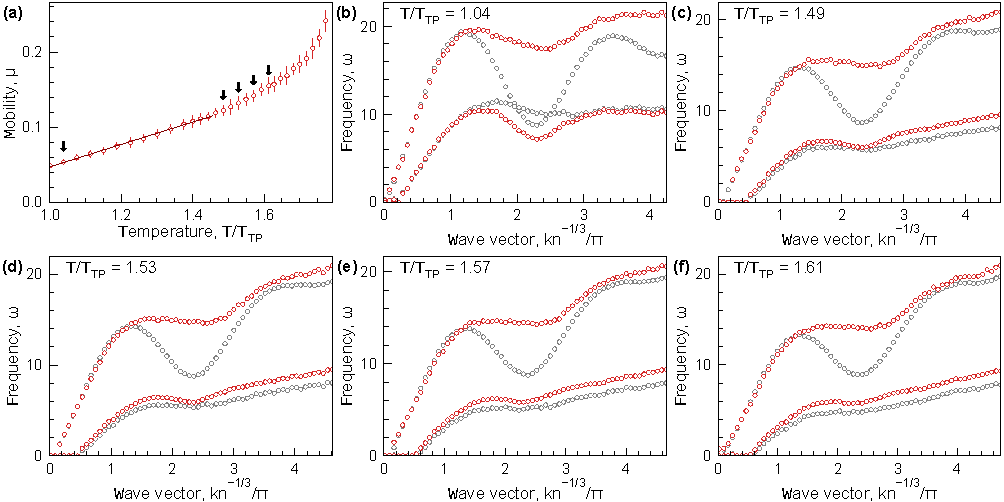
\includegraphics[width=170mm]{MACR-Figure4.pdf}
 \caption{(a) Температурная зависимость подвижности системы LJ$12$-$6$ вдоль жидкостной бинодали.
  Температуры, при которых рассчитывались спектры возбуждения, указаны черными стрелками.
  (b) - (f) спектры возбуждения LJ$12$-$6$ систем.
Спектры рассчитывались путем анализа скорости течения (уравнение~\eqref{MACR-eq7}) так же, как в Ref.~\cite{10.1038/s41598-019-46979-y}.
  Красный цвет соответствует гибридным модам, серый — результатам анализа отдельных мод~\cite{10.1038/s41598-019-46979-y}.
  В левом верхнем углу указаны пониженные температуры.}
\label{MACR-Figure4}
\end{figure}

\section{Результаты}
\label{MACR-SecResults}

Результаты расчета границ сосуществования газа и жидкости показаны на рис.~\ref{MACR-Figure3}(а).
Цветные точки обозначают бинодали, треугольники соответствуют срединным точкам.
Точки, которые использовались для аппроксимации [с использованием уравнения~(\ref{MACR-eq4})], выделены сплошной серой линией.
Экстраполированные бинодали обозначены пунктирной серой линией.
Для каждой рассматриваемой системы температура и плотность выражаются в единицах температуры и плотности тройной точки соответственно.
Последние значения вместе с параметрами критических точек приведены в Таб.~\ref{MACR-Table2}.

% \begin{table}[h!]
%     \centering{
%     \begin{tabular}{C{1.5cm}|C{1.0cm}|C{1.0cm}|C{1.0cm}|C{1.0cm}|C{1.0cm}|C{1.0cm}}
%         LJn-m & $T_{\rm CP}$ & $\rho_{\rm CP}$ & $T_{\rm TP}$ & $\rho_{\rm TP}$ & $A$ & $a$ \\ \hline
%         LJ12-4 & 4.85 & 0.291 & 1.75 & 0.952 & 0.559 & 0.107 \\
%         LJ12-5 & 2.18 & 0.304 & 1.03 & 0.867 & 0.804 & 0.208 \\
%         LJ12-6 & 1.29 & 0.315 & 0.72 & 0.830 & 1.002 & 0.326 \\
%         LJ16-6 & 1.55 & 0.316 & 0.98 & 0.816 & 0.969 & 0.334 \\
%         Ethane & 305.3 & 206.7 & 90.34 & 651.9 & 113.1 & 1.158
%     \end{tabular}
%
%     }
%     \caption{\textcolor{red}{
%     The values of densities and temperatures of critical and triple points and parameters of fits by Eq.~\eqref{MACR-eq4} for considered models.}
%     For generalized LJ systems temperatures and densities are given in reduced units. For ethane temperatures are in K and densities are expressed in $\text{kg}/\text{m}^3$. Critical and triple point parameters for ethane are taken from Ref.~\cite{10.1063/1.555785}.}
%     \label{MACR-Table2}
% \end{table}

Замечено, что с увеличением дальнодействующего характера потенциала температуры тройной и критической точек, а также их отношение $T_{\rm CP}/T_{\rm TP}$ также увеличивать.

Затем по рассчитанным фазовым диаграммам рассчитывали подвижность частиц при плотностях и температурах, соответствующих бинодали жидкости. Полученная зависимость подвижности частиц от температуры представлена на рис.~\ref{MACR-Рисунок 3}(b). Цветные точки на (b) соответствуют цветным точкам на (a). Серые точки обозначают подвижности на экстраполированных частях бинодали.

Заметим, что при низких температурах подвижность на бинодали имеет линейную зависимость от температуры. Его наклон увеличивается с уменьшением дальнодействующего характера потенциала взаимодействия (т. е. с увеличением показателя притяжения). Линейная зависимость сохраняется до определенной температуры, а затем становится нелинейной. Возникновение такой нелинейности может быть связано с особенностями коллективной динамики частиц, которые должны коррелировать со спектрами коллективных возбуждений.

Расчетные спектры системы LJ$12$-$6$ показаны на рис.~\ref{MACR-Figure4}. На рис.~\ref{MACR-Figure4}(а) показана зависимость подвижности от температуры, а черными стрелками указаны температуры, при которых рассчитывались спектры. Мы выбрали несколько точек вблизи температуры, при которой наблюдается начало нелинейной зависимости, и одну температуру вблизи тройной точки. На рис.~\ref{MACR-Figure4}(b)-(f) показаны расчетные соотношения дисперсии продольных и поперечных мод в этих точках. Красный цвет соответствует модели с двумя осцилляторами, а серый — одномодовому анализу~\cite{10.1038/s41598-019-46979-y}.

Нетрудно заметить, что по мере приближения температуры к точке, соответствующей возникновению нелинейной зависимости, дисперсионные соотношения демонстрируют переход от осциллирующей к монотонной зависимости от волнового числа. Таким образом, качественное изменение температурной зависимости подвижности частиц сопровождается количественным изменением спектров возбуждения. Наблюдаемая картина не является специфической для системы LJ$12$-$6$. Аналогичная тенденция наблюдается и для других исследованных обобщенных ЛД-систем (спектры их коллективных возбуждений см. в Приложении). Это дает новое свидетельство тесной связи между переносом жидкости и свойствами коллективного возбуждения.

\section{Заключение главы}
\label{MACR-SecConclusions}

В настоящей работе исследовано влияние формы потенциала парного взаимодействия на фазовые диаграммы и подвижность частиц в жидкой фазе. Были рассчитаны кривые сосуществования газа и жидкости для потенциалов с переменной относительной силой притяжения. Было замечено, что с увеличением дальнодействующего характера потенциала температуры тройной и критической точек, а также их отношение $T_{\rm CP}/T_{\rm TP}$ также увеличивать. Коэффициент диффузии и обратный ему коэффициент подвижности вычислялись на жидких бинодалиях. Обнаружено, что температурная зависимость подвижности линейна в широком диапазоне температур с тем большим наклоном, чем меньше диапазон притяжения. Кроме того, установлено, что начало нелинейной температурной зависимости подвижности при высоких температурах совпадает с переходом дисперсионных зависимостей коллективных возбуждений от осциллирующей к монотонной зависимости от волнового числа. Эти результаты открывают возможности для дальнейшего изучения диффузии и ее связи с коллективными процессами в конденсированных многочастичных системах.


\begin{figure}
\centering
 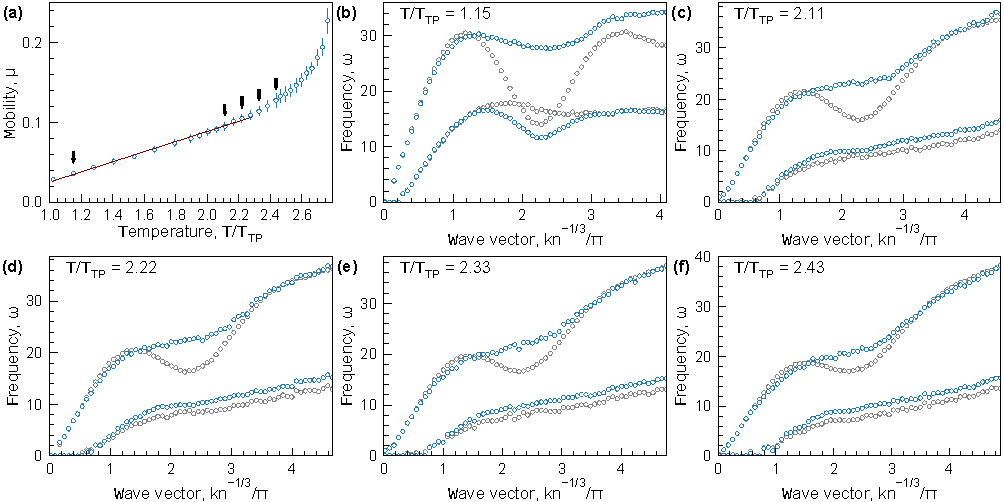
\includegraphics[width=150mm]{MACR-Figure5.pdf}
 \caption{Результаты для потенциала LJ$12$-$4$. Рисунок аналогичен рисунку~\ref{MACR-Figure4}(a)-(f).}
\label{MACR-Figure5}
\end{figure}


\begin{figure}
\centering
 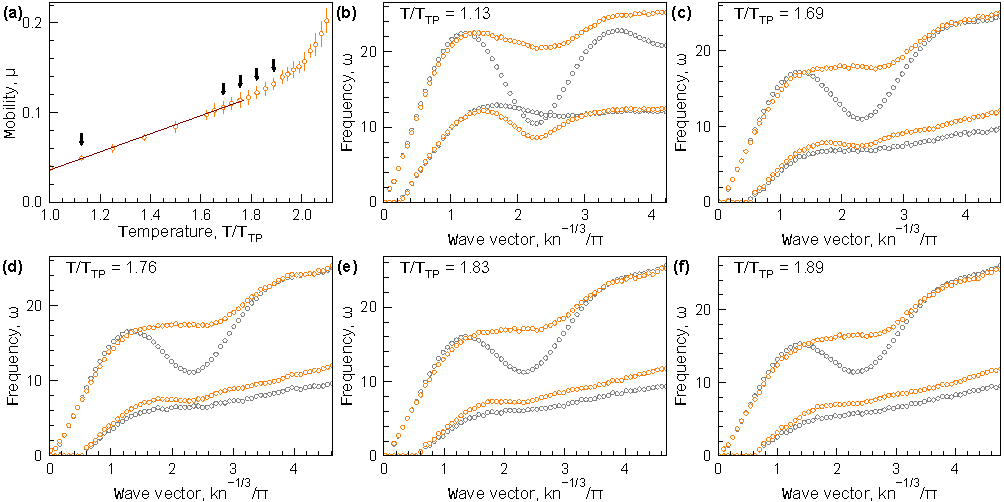
\includegraphics[width=150mm]{MACR-Figure6.pdf}
 \caption{Результаты для потенциала LJ$12$-$5$. Рисунок аналогичен рисунку~\ref{MACR-Figure4}(a)-(f).}
\label{MACR-Figure6}
\end{figure}


\begin{figure}
\centering
 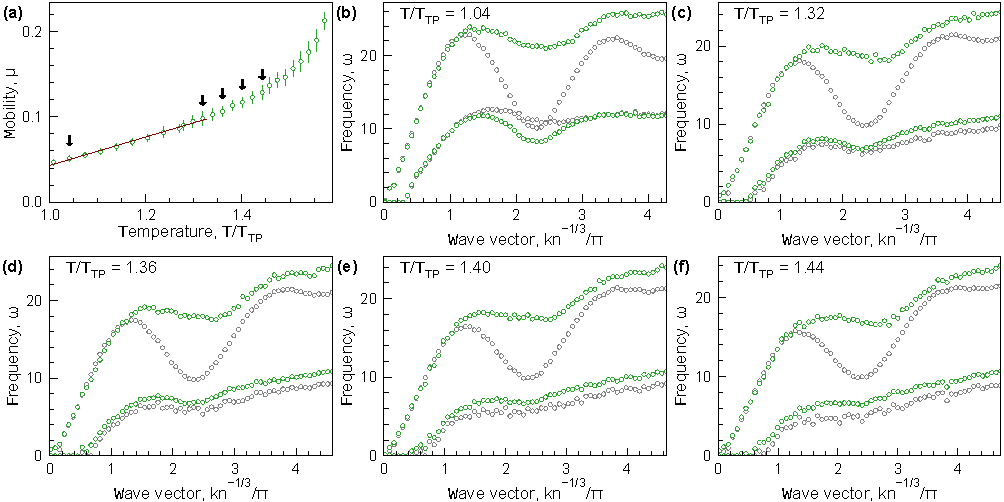
\includegraphics[width=150mm]{MACR-Figure7.pdf}
 \caption{Результаты для потенциала LJ$16$-$6$. Рисунок аналогичен рисунку~\ref{MACR-Figure4}(a)-(f).}
\label{MACR-Figure7}
\end{figure}


\begin{center}
\textbf{\large 4. ВЛИЯНИЕ ДАЛЬНОДЕЙСТВИЯ СИЛЫ ПРИТЯЖЕНИЯ НА СКОРОСТЬ НУКЛЕАЦИИ}
\end{center}
\refstepcounter{chapter}
\addcontentsline{toc}{chapter}{4. ВЛИЯНИЕ ДАЛЬНОДЕЙСТВИЯ СИЛЫ ПРИТЯЖЕНИЯ НА СКОРОСТЬ НУКЛЕАЦИИ}

\section{Введение}
\label{PRIMe-SecIntroduction}

Построение фазовых диаграмм различных систем является крайне важным для многих направлений науки и техники.
На данный момент удобным инструментом для изучения фазовых состояний веществ на уровне отдельных частиц является метод молекулярной динамики~\cite{10.1063/1.1730376, 10.1006/jcph.1995.1039} и модельных систем.
Примером служат пылевая плазма и коллойдные частицы во вращающихся электрических и магнитных полях~\cite{10.1038/s41598-017-14001-y, 10.1103/physreve.103.022608, 10.1103/physreve.96.043201}.
Для построения фазовых диаграмм систем существует несколько способов расчета, которые основаны на знании координат частиц в каждый момент времени.
К ним относятся термодинамическое интегрирование~\cite{10.1088/0953-8984/21/46/465104}, кластеризация с помощью разбиения на ячейки Вороного~\cite{10.1021/acs.jpcc.7b09317} и метод вычисления плотности газа и конденсата с помощью расчета профиля плотности системы с зафиксированными в пространстве газовой и конденсированной фазами~\cite{10.1021/jp806127j, 10.1021/jp1117213}.

Однако каждый из этих методов имеет ряд недостатков, которые не позволяют им быть универсальным способом для расчета фазовых диаграмм различных веществ ввиду большого количества параметров для настройки метода или неприменимости метода к кластерам произвольной формы.
Препятсвием также выступает высокая сложность алгоритма.

Упомянутые проблемы могут быть решены с помощью алгоритма кластеризации данных DBSCAN, ранее не применяемый к молекулярным системам, но продемонстрировавший хорошие результаты.
Так были созданы условия для изучения плавления и нуклеации веществ, а также для развития многих других областей, в которых внимание уделяется и модельным системам и МД моделирования.


\section{Методы}
\label{PRIMe-SecMethods}

\subsection{Алгоритм кластеризации данных DBSCAN как классификатор частиц в двухфазных системах}
\label{PRIMe-SubSecDBSCAN}

Для решения задачи классификации частиц в двухфазных системах был выбран алгоритм кластеризации DBSCAN.
Выбор метода обусловлен тем, что он позволяет классифицировать систему на кластеры данных и выбросы, что в рамках задачи распознавания фаз можно интепретировать как конденсат и газ соответственно.

Для корректной работы данного алгоритма кластеры должны быть одинаковой плотности, что в нашем случае соответствует кластерам, находящимся в термодинамическом равновесии друг с другом.
Такой алгоритм естественным образом легко адаптировать как к двумерным, так и к трехмерным системам частиц, благодаря чему его можно применять в широком диапазоне задач.

DBSCAN требует задания двух параметров: $\varepsilon$-окрестность и минимального числа точек $k$, которые должны образовывать плотную область~\cite{schubert2017dbscan}.
Алгоритм начинается с произвольной ещё не просмотренной точки.
Выбирается $\varepsilon$-окрестность точки и, если количество содержащихся в ней точек больше или равно $k$, изначальная точка помечается как кластер, в противном случае же -- как поверхность или шум.

Если точка найдена как плотная точка кластера, то ее $\varepsilon$~-~окрестность также является частью этого кластера.
Следовательно, все точки, найденные в $\varepsilon$~-~окрестности этой точки, добавляются к кластеру.
Этот процесс продолжается, пока не будет найден связный по плотности кластер.
Затем выбирается и обрабатывается новая непосещённая точка, что ведет к обнаружению следующего кластера или шума (газовых точек).
Следующим шагом точки кластера, не содержащие в своей $\varepsilon$~-~окрестности $k$ или больше соседей, помечаются как точки поверхности.
Принцип кластеризации показан на рисунке~\ref{kepsilon}.

DBSCAN может быть использован с любой функцией расстояния~\cite{schubert2017dbscan} (а так же с функцией похожести или логическим условием)~\cite{10.1023/a:1009745219419}.
Функция расстояния может рассматриваться как дополнительный параметр.
В рамках анализа двухфазной системы частиц в качестве функции расстояния используется норма Евклидового пространства.

Новый алгоритм классификации частиц, основанный на DBSCAN, разделяет систему на 3 класса (на конденсат, газ и поверхность).
Частица считается основной (конденсат), если в ее окрестности $\varepsilon$ находится не меньше $k$ частиц.
Параметр $k$ играет в нашем случае также роль минимального значения размера кластеров в системе.
Частица считается поверхностной, если она соседствует с любой из основных частиц, но при этом не имеет нужное количество соседей, чтобы считаться основной.
Выбросом, то есть газом, являются частицы, которые не соседствуют с основными частицами.
Пример деления системы на три класса представлен на рисунке~\ref{DBSCAN-Illustr}(c).

\begin{figure}[!t]
    \centering
    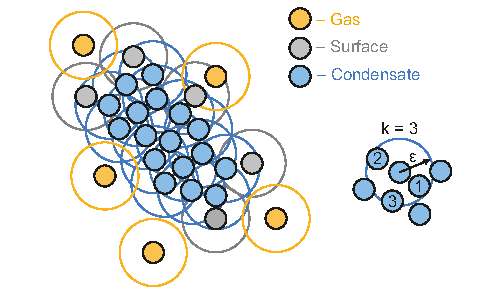
\includegraphics[width=140mm]{kepsilon.pdf}
    \caption{Принцип работы алгоритма кластеризации DBSCAN для случая $k = 3$.
    Синие точки являются основными точками (конденсатом), поскольку область с радиусом $\varepsilon$, окружающая эти точки, содержит по меньшей мере трех соседей (не считая саму точку).
    Серые точки не имеют в своей $\varepsilon$~-~окрестности трех соседей, но имеют покрайней мере одну основную точку (частицу конденсата).
    Такие точки относятся к поверхности.
    У ораневых точек в своей $\varepsilon$~-~окрестности нет ни одной основной точки, поэтому они считаются частицами газа.}
    \label{kepsilon}
\end{figure}

Важным вопросом применения данного алгоритма является выбор оптимальных значений параметров $\varepsilon$ и $k$.
В качестве функции расстояния мы используем норму Евклидова пространства, но выбор $\varepsilon$ и $k$ не так очевиден.

В задачах классификации выбор значения $\varepsilon$ часто выполняется автоматически и зависит только от $k$.
Для каждой точки данных вычисляется расстояние до самой дальней из $k$ ближайших точек.
Полученные расстояния сортируются.
На графике зависимости данного расстояния от индекса массива отсортированных точек наблюдается точка перегиба, которая определяет оптимальное значение параметра $\varepsilon$.
Наиболее эффективным способом получения такой точки является нахождение точки, наиболее удаленной от прямой, соединяющей минимальное и максимальное значение расстояния.
Выбор оптимальных параметров иллюстрируется на рисунке~\ref{epsilon_k}.

Обнаружено, что для рассматривоемой физической задачи данный метод также подходит, поэтому единственным свободным параметром в используемом алгоритме остается значение $k$, которое имеет смысл минимального значения размера кластера, и как будет показано далее, может быть взято в большом диапазоне значений, а малое изменение данного параметра слабо влияет на результат классификации, что делает работу выбранного метода более стабильной.
Пример кластеризации системы частиц после применения алгоритма DBSCAN представлен на рисунке \ref{DBSCAN-Illustr}(a).

\begin{figure}[!t]
    \centering
    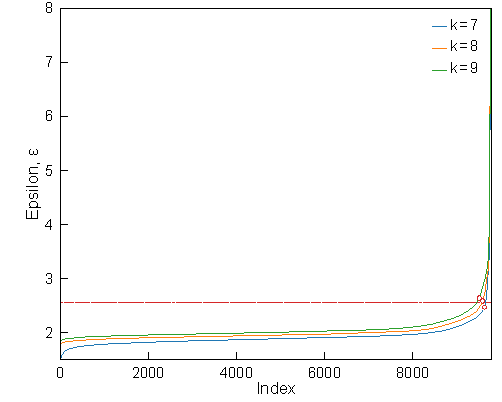
\includegraphics[width=150mm]{Figure0.pdf}
    \caption{Выбор оптимального параметра $\varepsilon$.
    Красным цветом указаны точки для различных значений параметра $k$, наиболее удаленные от линии, соединяющей начало и конец кривой расстояний.}
    \label{epsilon_k}
\end{figure}

Классификация частиц поверхности в зависимости от задачи может различаться.
При необходимости отнесения к поверхности минимального количества частиц поверхностью считаются только те частицы, которые относятся к конденсату, не будучи основными (по условию k-NN < k).
Данное выделение поверхности представлено на рисунке~\ref{DBSCAN-Illustr}(b).
Однако при необходимости выделения поверхности, полностью ограничивающей кластер, может быть применен алгоритм выделения поверхности.
Алгоритм выделения поверхности следующий: набору точек можно присвоить многоугольник с помощью набора кругов определенного радиуса, для этого вокруг точек рисуется произвольная форма, у которой удаляется как можно большая часть, используя круги определенного радиуса.
Этот процесс продолжается достаточно долго, не замыкая ни одной точки.
Малый радиус означает, что можно удалить больше частиц, больший радиус -- меньшее <<удаление>>.
Т.е. малый радиус создает плотную обрезанную форму, тогда как бесконечный радиус воссоздает выпуклую оболочку набора.
Точки, определенные как краевые, затем соединяются прямыми гранями, что может создать пустые области внутри набора точек.
Система, после применения данного алгоритма выделения поверхности представлена на рисунке~\ref{DBSCAN-Illustr}(c).

\begin{figure}[!t]
    \centering
    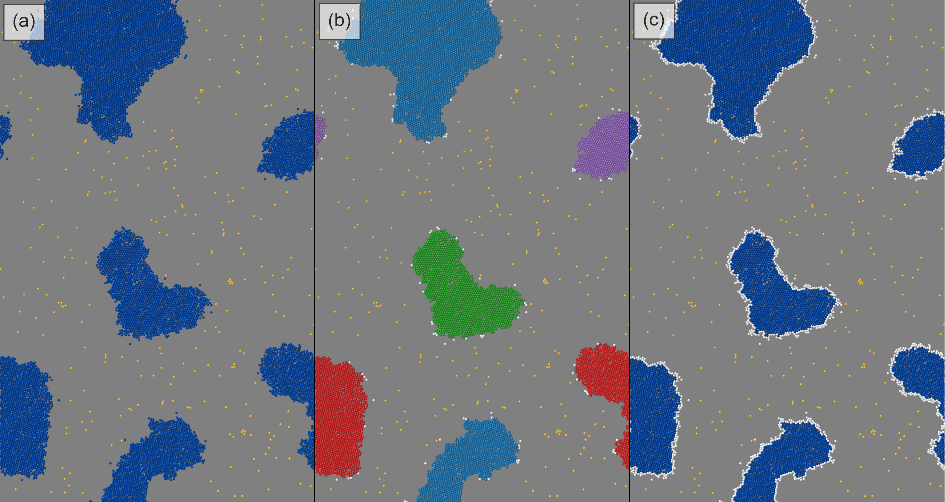
\includegraphics[width=\linewidth]{PRIMe-Figure104.pdf}
    \caption{Пример распознавания частиц в 2D системе LJ12-6. 
    (a) Результат работы метода DBSCAN (классификация частиц на конденсат и газ). 
    (b) Пример выделения частиц поверхности, по условию принадлежности к конденсату, а не к основным частицам.
    Разные кластеры раскрашены в разные цвета с учетом регулярных граничных условий. 
    (с) Пример выделения регулярной поверхности, охватывающей все частицы кластера.}
    \label{DBSCAN-Illustr}
\end{figure}

Данный метод легко обобщается на трехмерные системы.
Пример классификации частиц в трехмерном моделировании с потенциалом Леннарда-Джонса 12-6 изображен на рисунках \ref{D3_flat_layer} и \ref{D3_free_conf}.

\begin{figure}[!t]
    \centering
    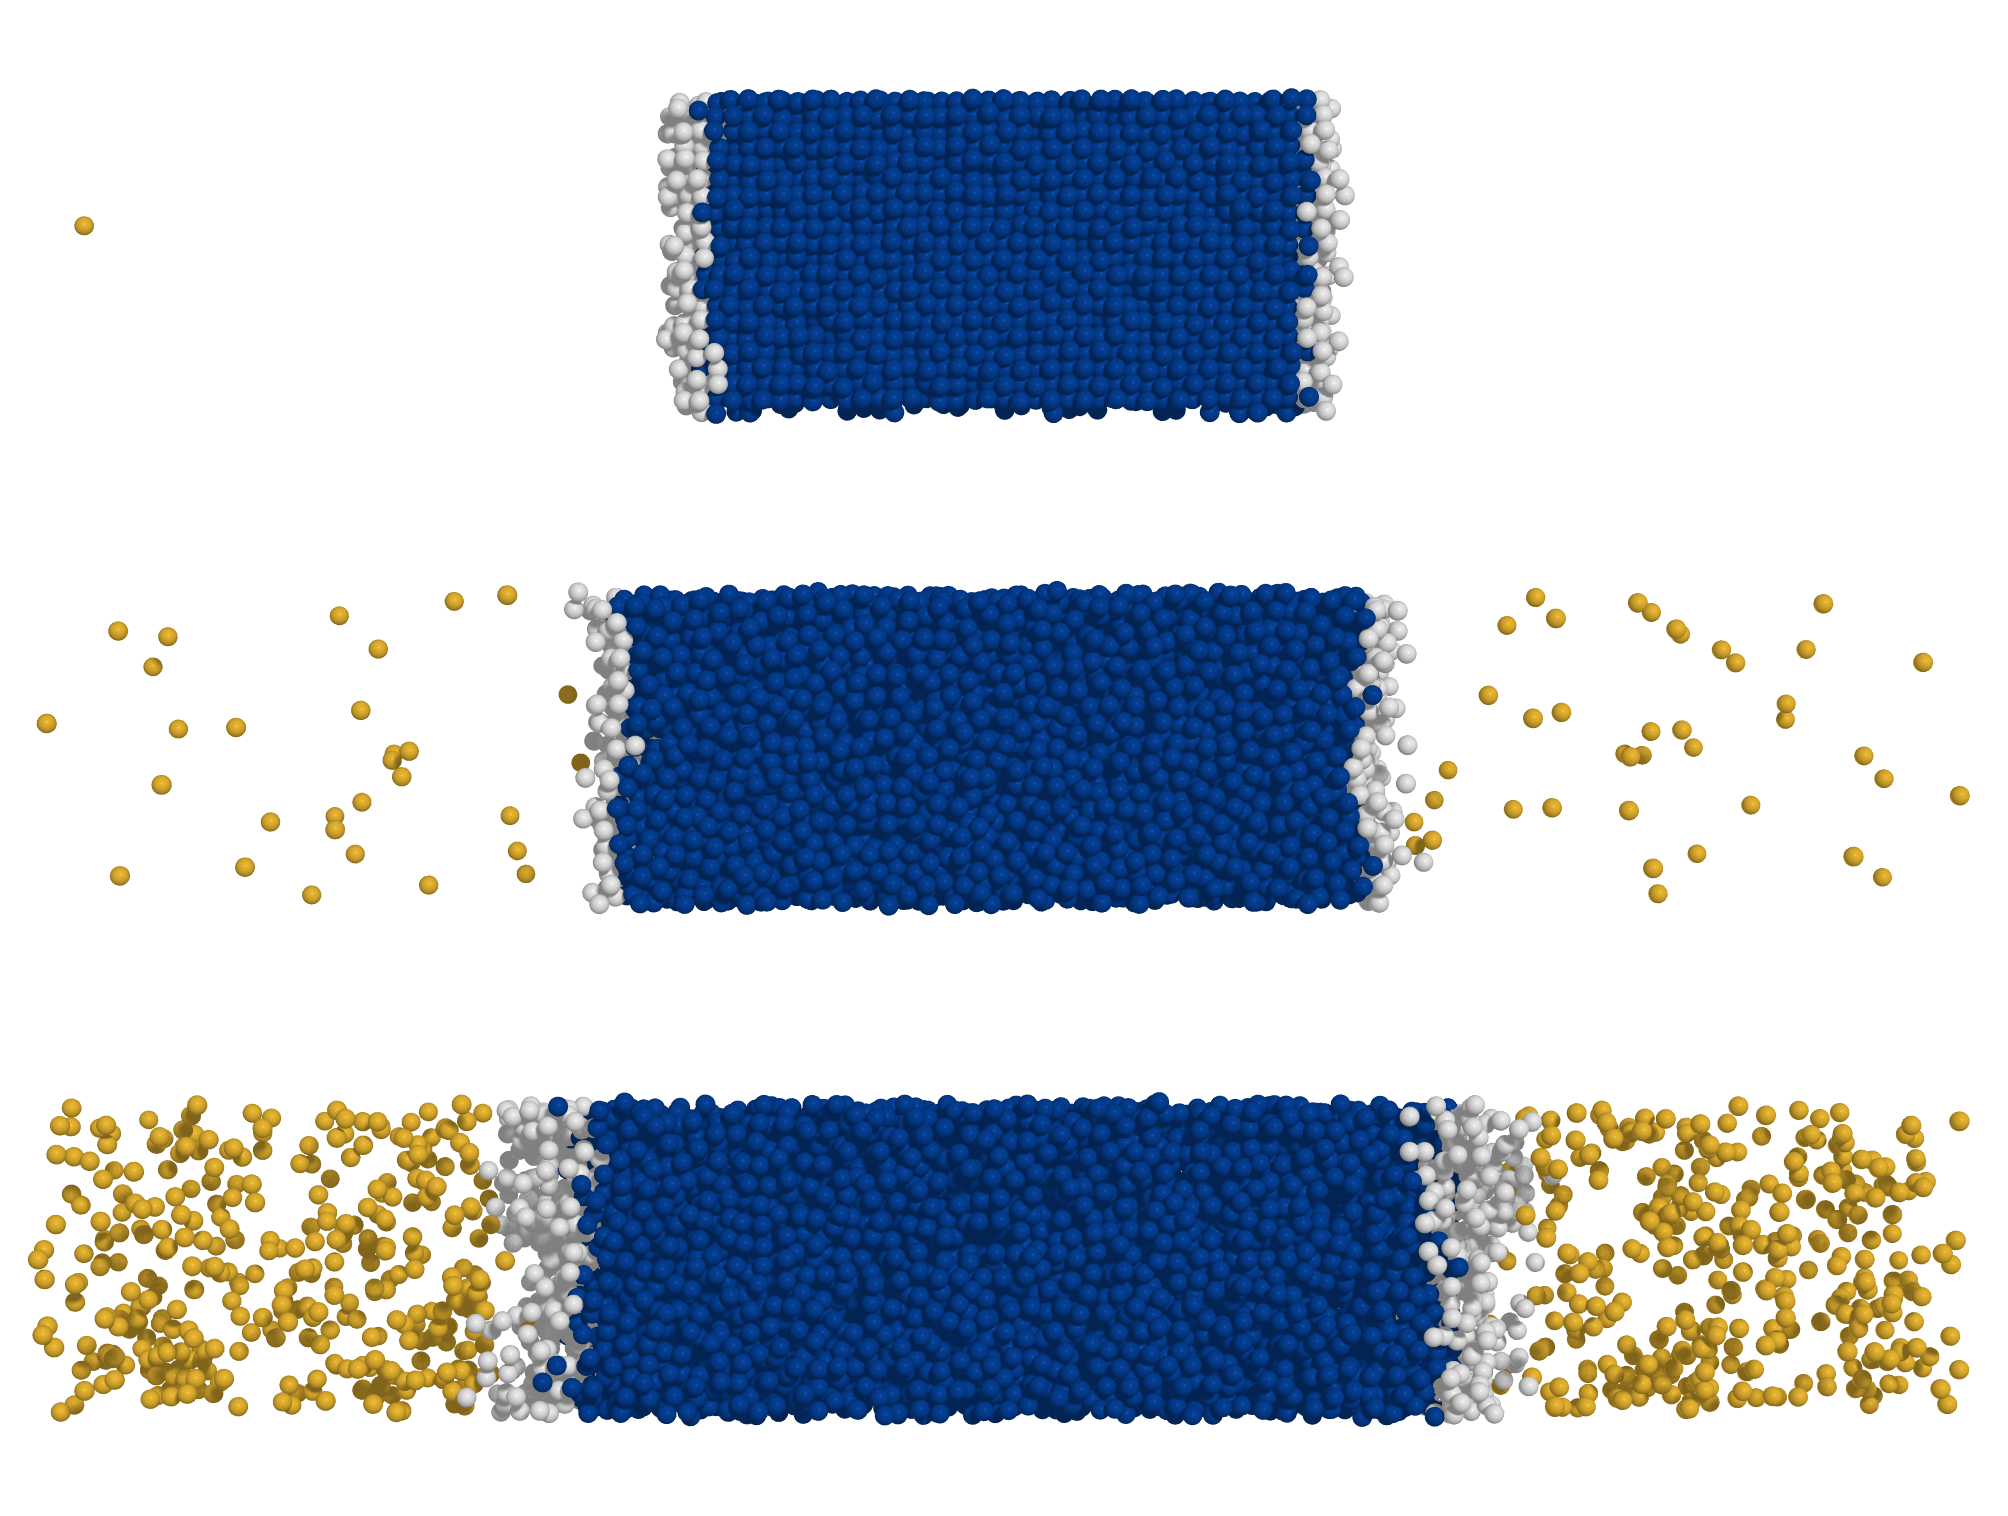
\includegraphics[width=\linewidth]{PRIMe-Figure101.png}
    \caption{Распознавание фаз методом DBSCAN в 3D системе LJ12-6 в случае плоского слоя для разных температур.}
    \label{D3_flat_layer}
\end{figure}


\begin{figure}[!t]
    \centering
    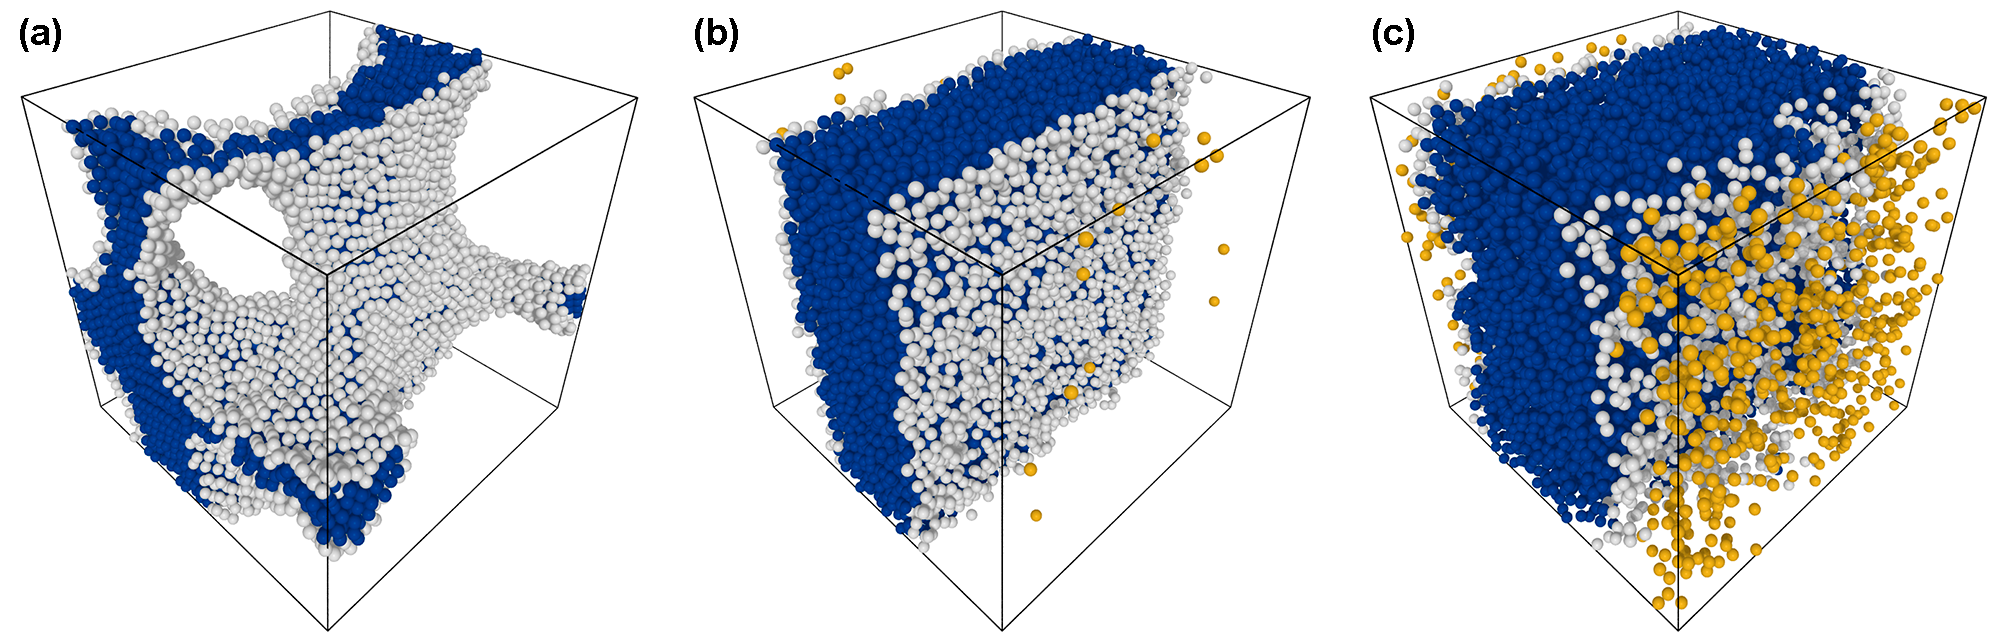
\includegraphics[width=\linewidth]{PRIMe-Figure103.png}
    \caption{Распознавание фаз для кластера произвольной формы в трехмерной системе LJ12-6 при различной температуре: (a) кластер произвольной формы при температуре ниже тройной точки; (b) система в состоянии жидкость + газ; (с) система вблизи критической точки.}
    \label{D3_free_conf}
\end{figure}



\subsection{Построение фазовых диаграмм}
\label{PRIMe-SubSecPhaseDiagram}

Новый метод классификации частиц на фазы дает возможность использовать уникальный подход к построению фазовых диаграмм, который основан на вычислении плотности подсистем, содержащих только частицы определенной фазы.
Для демонстрации работы рассматриваемого метода классификации и построения фазовых диаграмм были проведены МД-моделирования в NVT ансамбле системы частиц, взаимодействующих по обобщенному потенциалу Леннарда-Джонса (LJn-m):

\begin{equation}
U_{n-m}(r)=4 \varepsilon\left[\left(\frac{\sigma}{r}\right)^{n}-\left(\frac{\sigma}{r}\right)^{m}\right]
\label{MACR-eq1}
\end{equation}
где $\epsilon$ и $\sigma$ -- магнитуда и характерный масштаб отталкивания соответственно.
Были использованы нормированная температура $ T/ \epsilon \rightarrow T $, расстояние $ r/ \sigma \rightarrow r $ и плотность частиц $ \rho \sigma ^ 3 / m \rightarrow n$ (здесь $ m $ - масса частицы). 

В качестве примеров выступили потенциалы LJ12-4, LJ12-5, \\ LJ12-6, LJ16-6, в случае трехмерных систем, и LJ12-3, LJ12-4, LJ12-5, LJ12-6, LJ12-7, в случае двумерных.

После классификации системы на конденсат и газ и поверхность могут быть применены данные для различных расчетов, например, для вычисления фазовые диаграммы веществ.

Для этого случайным образом вся система разбивается на подобласти, после чего расчитываются их плотности как $\rho_i = N / V$, где $N$ -- количество частиц попавших в сферу (окружность для 2D случая) радиусом $\varepsilon$; $V$ -- объем сферы радиусом $\varepsilon$ (площадь окружности в 2D случае); $i$ -- индекс области.

Затем случайно выбранные области относятся к конденсату или газу по следующим критериям:
\begin{enumerate}
    \item Если в области $\varepsilon$ находятся только частицы конденсата и их не меньше чем $k$, то эта область является конденсатом;
    \item Если в область попали частицы поверхности, то эта область относится к поверхности и не участвует в статистике плотностей газа и конденсата;
    \item Если в область попали только газовые частицы или в области нет частиц, то эта область считается занимаемой газом.
\end{enumerate}
Затем рассчитываются плотности соответствующих областей и вычисляются среднее значение плотности конденсата и газа.

Для расчета фазовых диаграмм вещества в координатах $\rho$-$T$ необходимо знать плотность газа и конденсата при соответствующих температурах.
Для этого в начале моделирования берется температура существенно ниже тройной точки, затем система релаксирует.
После релаксации температура системы начинает медленно линейно повышаться от температуры релаксации до закритической.
Нагревание происходит медленно, поэтому систему в каждый момент времени можно считать находящейся в состоянии термодинамического равновесия, что позволяет быстро найти для каждой температуры соответствующие плотности конденсата и газа усреднив их по нескольким соседним кадрам моделирования.

\begin{figure}[!t]
    \centering
    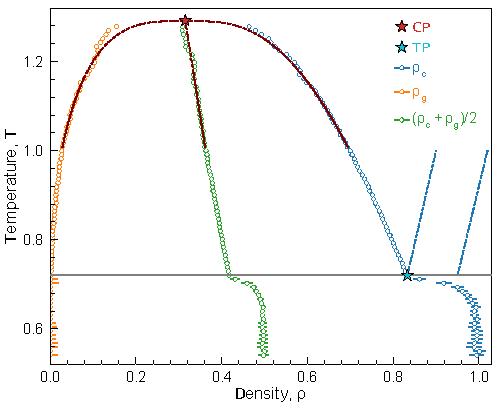
\includegraphics[width=150mm]{MACR-Figure2.pdf}
    \caption{Фазовая диаграмма системы LJ12-6, изображенной на рисунке~\ref{D3_free_conf}.
    Оранжевые и синие символы — плотности газа и конденсата, полученные путем усреднения плотности областей, соответствующих конденсату и газу.
    Зеленые символы -- медиана $\rho_m=(\rho_g+\rho_c)/2$.
    Сплошная красная линия соответствует уравнению ~\eqref{MACR-eq4}.
    Тройные и критические точки обозначены синими и красными звездочками соответственно.}
    \label{phase_diagram}
\end{figure}


\begin{table}[h!]
    \centering{
    \begin{tabular}{l|l|l|l|l|l|l}
        Потенциал & $T_{\rm CP}$ & $\rho_{\rm CP}$ & $T_{\rm TP}$ & $\rho_{\rm TP}$ & $A$ & $a$ \\ \hline
        \multicolumn{7}{c}{3D системы:} \\ \hline
        LJ12-4 & 4.416 & 0.278 & 1.500 & 0.980 & 0.578 & 0.128 \\
        LJ12-5 & 2.080 & 0.301 & 1.030 & 0.900 & 0.846 & 0.251 \\
        LJ12-6 & 1.282 & 0.308 & 0.645 & 0.865 & 1.002 & 0.385 \\
        LJ16-6 & 1.532 & 0.309 & 0.900 & 0.850 & 0.987 & 0.412 \\ \hline
        \multicolumn{7}{c}{2D системы:} \\ \hline
        LJ12-3 & 2.697 & 0.304 & 1.080 & 0.820 & 0.702 & 0.117 \\
        LJ12-4 & 1.170 & 0.350 & 0.700 & 0.792 & 0.823 & 0.150 \\
        LJ12-5 & 0.732 & 0.356 & 0.530 & 0.775 & 0.924 & 0.326 \\
        LJ12-6 & 0.517 & 0.355 & 0.405 & 0.780 & 0.982 & 1.019 \\
        LJ12-7 & 0.371 & 0.363 & 0.316 & 0.780 & 1.058 & 1.680 \\ \hline
    \end{tabular}
    }
    \caption{Значения тройных и критических точек, а также коэффициентов фитирования $A$ и $a$ из уравнений \eqref{MACR-eq4} для двумерных и трехмерных систем Леннарда-Джонса, рассматриваемых в данной работе.}
    \label{PRIMe-Table2}
\end{table}



Вблизи критической температуры вычисление плотностей газа и конденсата становится затруднительным из-за растущих флуктуаций плотности в системе.
Поэтому для более точного определения критической температуры фазовые диаграммы можно аппроксимировать следующими уравнениями~\ref{MACR-eq4}.

В трехмерии для потенциала LJ12-6 критический индекс $\beta_c = 0.325$, а в двумерии -- $\beta_c = 0.5$.
Пример построения фазовой диаграммы для трехмерной системы LJ12-6 и нахождение тройной и критической точки изображено на рисунке~\ref{phase_diagram}.

Главным достоинством такого подхода к построению фазовых диаграмм по сравнению с методами <<плоского слоя>>~\cite{10.1021/jp806127j, 10.1021/jp1117213} и термодинамическим интегрированием~\cite{10.1088/0953-8984/21/46/465104} является нечувствительность метода к форме кластеров, а также произвольное начальное и последующее расположение частиц, скорость работы алгоритма благодаря автоматизации выбора параметров и расчетов.



\subsection{Детали МД-моделирований для построения фазовых диаграмм}
\label{PRIMe-SubSecPhaseDiagramMD}



Все МД-симуляции были выполнены в ансамбле NVT (N, V и T -- количество частиц, объем системы и температура) с периодическими граничными условиями при использовании пакета моделирования \\  LAMMPS~\cite{10.1006/jcph.1995.1039}.
Исходное состояние системы формировалось следующим образом: (i) кубический ящик (квадратный в 2D случае) моделирования заполнялся равновесным кристаллом (в данном случае ГЦК) из $N$ частиц со средней плотностью системы $\rho_a$; (ii) система релаксировала на протяжении $3 \times 10^5$ шагов при температуре $T_{start}$.
Результирующее начальное состояние для 3D системы LJ12-6 показано на рис.~\ref{D3_free_conf}(а).
Затем температура системы линейно увеличивалась от $T_{start}$ до $T_{stop}$ в течение $n_{step}$ шагов моделирования с временным шагом $\Delta t$.
Различия в моделированиях представленны в таблице \ref{MACR-Table1}.


\begin{table}[h!]
    \centering{
    \begin{tabular}{l|l|l|l|l|l|l}
        Потенциал & $\rho_a$ & $r_c$ & $T_{\rm start}$ & $T_{\rm stop}$ & $n_{step}$& $\Delta t$ \\  \hline
        \multicolumn{7}{c}{3D системы:} \\\hline
        LJ12-4 & \multirow{4}*{0.35} & 12.0 & 0.5 & 4.5 & \multirow{4}*{$5 \times 10^6$}  & \multirow{4}*{$5 \times 10 ^ {- 4}$} \\
        LJ12-5 &  & 10.0 & 0.2 & 2.5 & & \\
        LJ12-6 &  & 8.0 & 0.4 & 1.4 &  & \\
        LJ16-6 &  & 8.0 & 0.6 & 1.6 &  & \\ \hline
        \multicolumn{7}{c}{2D системы:} \\\hline
        LJ12-3 & \multirow{5}*{0.35} & 15.0 & 0.5 & 3.0 & \multirow{5}*{$7 \times 10^6$}  & \multirow{5}*{$5 \times 10 ^ {-4}$} \\
        LJ12-4 &  & 15.0 & 0.4 & 1.4 & & \\
        LJ12-5 &  & 10.0 & 0.2 & 0.9 &  & \\
        LJ12-6 &  & 8.0 & 0.35 & 0.55 &  & \\
        LJ12-7 &  & 8.0 & 0.28 & 0.4 &  & \\ \hline
    \end{tabular}
    }
    \caption{Параметры, используемые в МД-моделировании для бимодальных расчетов:
    где $\rho$ — средняя плотность системы, $r_c$ — радиус отсечки,
    $T_{start}$ и $T_{stop}$ — начальная и конечная температуры моделирования,
    $n_{step}$ — количество шагов моделирования, а
    $\Delta t$ — временной шаг.}
    \label{MACR-Table1}
\end{table}


\section{Результаты}
\label{PRIMe-SecResults}

\subsection{Результаты построения фазовых диаграмм}
\label{PRIMe-SubSecPhaseDiagramMD}

На рисунке \ref{phase_diagram}(a) и \ref{phase_diagram}(b) представленны результаты построения фазовых диаграмм для двумерия и трехмерия соответственно, расчитанные с помощью нового метода классификации частиц на фазы.
Фазовые диаграммы нормированны на температуру и плотность тройной точки, представленные в таблице \ref{PRIMe-Table2}.

Как можно заметить, представленные фазовые диаграммы имеют незначительные погрешности плотности конденсата и газа.
Данный результат показывает большую стабильность по сравнению с другими методами построения фазовых диаграмм~\cite{10.1021/jp806127j, 10.1021/jp1117213}.
Важным достоинством нового метода является то, что для расчета не требуется множество моделирований как для метода термодинамического интегрирования~\cite{10.1080/00268976.2019.1699185}. Отметим, что для рассматриваемого метода также не требуется ни системы конкретной формы, ни моделирования плоского слоя~\cite{10.1021/jp806127j, 10.1021/jp1117213}.
В таблице~\ref{PRIMe-Table3} приведено сравнение методов построения фазовых диаграмм, включая новый.



\begin{table}[h!]
    \centering{
    \begin{tabular}{l|l|l|l|l}
        Метод & Форма & 3D & Скорость & Точность \\  \hline
        Представленный метод & \checkmark & \checkmark & \checkmark & \checkmark  \\
        Метод плоского слоя~\cite{10.1021/jp806127j, 10.1021/jp1117213} & $\times$ & \checkmark & \checkmark & $\times$  \\
        Термодинамическое интегрирование~\cite{10.1080/00268976.2019.1699185} & \checkmark   & \checkmark   & $\times$   & \checkmark    \\
        Метод основанный на $R^2$-параметре~\cite{10.1021/acs.jpcc.7b09317} & \checkmark & $\times$ & \checkmark & $\times$  \\ \hline
    \end{tabular}
    }
    \caption{Сравнение различных методов построения фазовых диаграмм.
    Под 2D и 3D понимается применимость данных методов в двумерных или трехмерных системах, под скоростью -- величина затраченого времени в человеко-часах на одну точку фазовой диаграммы относительно других представленных методов, под точностью -- точность метода относительно других представленных методов.}
    \label{PRIMe-Table3}
\end{table}



\begin{figure}[!t]
    \centering
    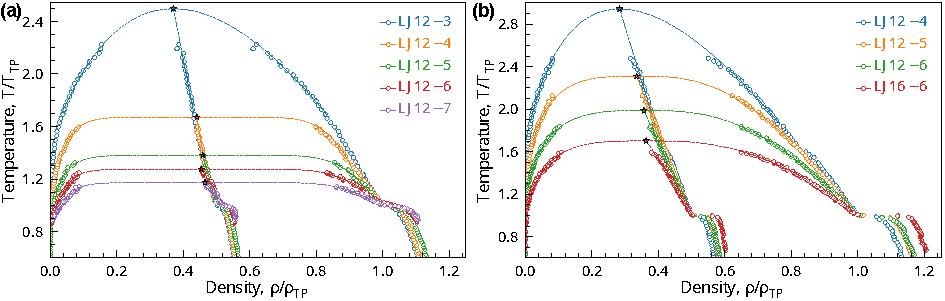
\includegraphics[width=\linewidth]{Figure11.pdf}
    \caption{Фазовые диаграммы систем с различным дальнодействием притяжения.
    (a) Фазовые диаграммы в двумерных системах.
    (b) Фазовые диаграммы в трехмерных системах.}
    \label{phase_diagram}
\end{figure}

\subsection{Тесты на устойчивость метода к плотности системы и входным параметрам}
\label{PRIMe-SubSecTests}


Для успешного применения данного алгоритма кластеризации необходимо выявить границы его применимости.
В связи с чем были проведены тесты на устойчивость метода к изменению начальной плотности системы и выбору минимального размера кластеров.

\begin{figure}[!t]
    \centering
    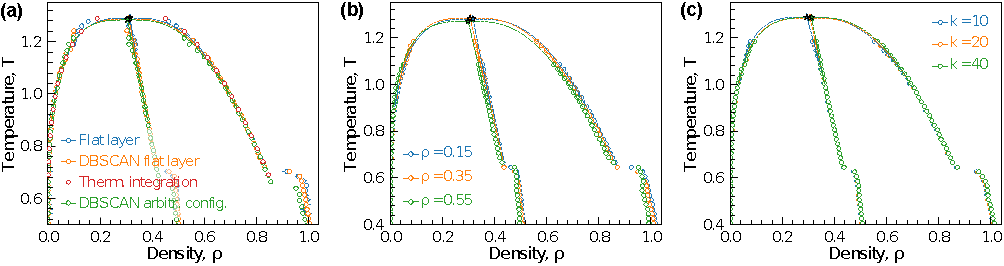
\includegraphics[width=\linewidth]{Figure10.pdf}
    \caption{\textbf{(a)} Сравнение различных методов построения фазовых диаграмм.
    Красным отмечен самый точный метод - термодинамическое интегрирование~\cite{10.1080/00268976.2019.1699185}.
             \textbf{(b)} Тест на влияние средней плотности на фазовую диаграмму системы LJ12-6 в трехмерии.
             \textbf{(c)} Тест на влияние начального параметра $k$ на фазовую диаграмму системы LJ12-6 в трехмерии.}
    \label{tests}
\end{figure}



На рисунке~\ref{tests}(b) представлен результат построения фазовых диаграмм систем с потенциалом взаимодействия LJ12-6 в трехмерии с различной начальной плотностью системы.
Примечательно, что существенное изменение плотности системы слабо влияет на расчет фазовых диаграмм и критических точек.



Кроме устойчивости к плотности системы данный алгоритм построения фазовых диаграмм также должен быть нечувствительным к изменению параметра $k$.
На рисунке~\ref{tests}(c) продемонстрирован тест на чувствительность метода к данному параметру.
Была смоделирована система с потенциалом LJ12-6 в трехмерии и новым методом расчета.
Фазовые диаграммы построены с использованием различных входных параметров $k$.
Анализ результатов показывает, что изменение параметра $k$ практически не влияет на фазовую диаграмму.


Для сравнения нового метода построения фазовых диаграмм с уже существующими была проведена обработка одного моделирования новым методом и методом <<плоского слоя>>~\cite{10.1021/jp806127j, 10.1021/jp1117213}.
Кроме того, было произведено сравнение полученных результатов с фазовой диаграммой системы с произвольной начальной формой кластера.
Результаты тестов приведены на рисунке~\ref{tests}(a), где синим цветом обозначена фазовая диаграмма вычисленная методом <<плоского слоя>>, оранжевым -- фазовая диаграмма, рассчитанная новым методом распознавания фаз.
На том же моделировании, что и <<плоский слой>>, зеленым цветом показана фазовая диаграмма вычисленная новым методом, только в данном случае на моделировании с произвольным начальным расположением частиц.
Красным цветом представленны данные, расчитанные методом термодинамического интегрировния, самым точным из представленных~\cite{10.1080/00268976.2019.1699185}.

Как можно заметить, фазовая диаграмма, построенная по моделированию, содержащему плоский слой частиц, оказалась практически идентичной для разных методов.
Новый метод создает более плавную фазовую диаграмму и меньшую погрешность плотности кристаллической фазы.
Однако при этом новый метод, примененный к системе с произвольным расположением частиц, дает несколько отличный результат от методов, примененных к плоскому слою частиц.
Это явление вызвано тем, что <<плоский слой>> частиц более стабильный и может находится в состоянии перегретого кристалла, в то время как на кластерах произвольной формы зародыши плавления начинают появляться при меньшей температуре.
Данный факт делает метод <<плоского слоя>> не таким универсальным, как новый метод классификации, основанный на DBSCAN, так как результирующие фазовые диаграммы полученные методом <<плоского слоя>> имеют завышенную тройную точку, в отличии от нового метода, который способен строить фазовую диаграмму для систем с произвольной формой.


\section{Изучения скорости нуклеации в переохлажденных системах}
\label{PRIMe-SecNucleation}

\begin{figure}[!t]
    \centering
    \includegraphics[width=\linewidth]{Otchet}
    \caption{Процесс зарождения и роста кластеров в переохлажденной системе частиц взаимодействующих посредством потенциала Леннарда-Джонса.}
    \label{otchet}
\end{figure}


\begin{figure}[!t]
    \centering
    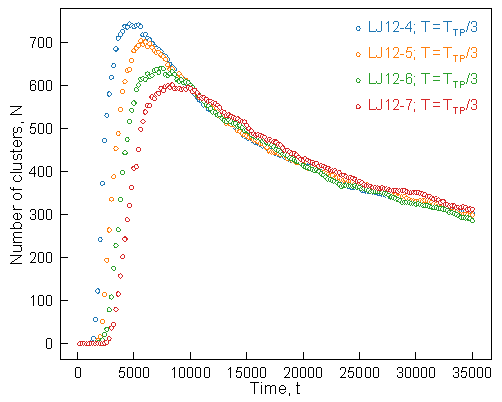
\includegraphics[width=150mm]{countCluster}
    \caption{Зависимость количества кластеров от времени.}
    \label{countCluster}
\end{figure}

\begin{figure}[!t]
    \centering
    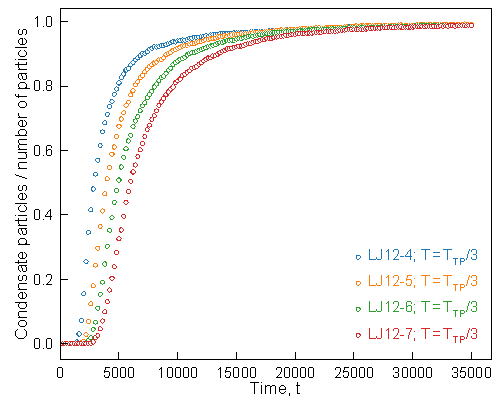
\includegraphics[width=150mm]{countParticles}
    \caption{Зависимость доли частиц, находящихся в конденсированном состоянии от времени для различных потенциалов.}
    \label{countParticles}
\end{figure}

\begin{figure}[!t]
    \centering
    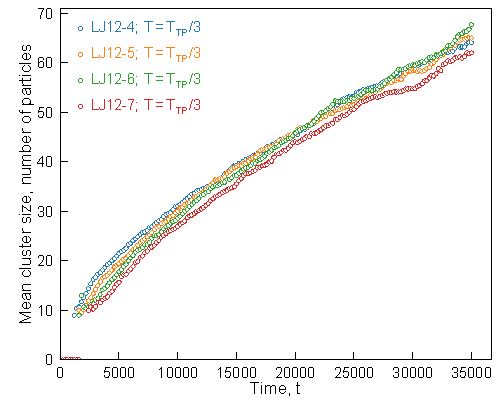
\includegraphics[width=150mm]{meanParticles}
    \caption{Зависимость среднего размера кластера от времени для систем с различным дальнодействием потенциала.}
    \label{meanParticles}
\end{figure}

Для демонстрации возможностей нового метода распознавания фаз было решено определить влияние дальнодействия потенциала на скорость нуклеации в системе с одинаковой степенью переохлаждения.

Для того, чтобы исключить влияние глубины потенциальной ямы на скорость нуклеации, был выбран нормированный потенциал из предыдущих работ~\ref{LJnm}.

При данном потенциале взаимодействия глубина остается постоянно равной единице, в то время как дальнодействие можно изменять варьируя степень притяжения $m$.

Для выяснения степени переохлаждения системы были вычислены температурные точки для двумерных систем $U_{12-4}$, $U_{12-5}$, $U_{12-6}$, $U_{12-7}$.
Значение температуры тройной точки определяется по резкому уменьшению плотности бинодали жидкость-газ.

Затем моделируются системы с равномерной плотностью распределения частиц и одинаковой степенью переохлаждения, то есть температура моделирования -- это $T = T_{TP} / a$, где в рамках нашей задачи $a = 3.0$, а $T_{TP}$ является температурой тройной точки и вычисляется на предыдущем шаге.

На рисунке~\ref{otchet} представлены снимки системы спустя разные отрезки времени после начала моделирования.
Новый алгоритм классификации на фазы позволяет наблюдать за процессами зарождения и последующего <<слипания>> кластеров.


На рисунке~\ref{countCluster} изображена временная зависимость количества кластеров в системах с различным дальнодействием притяжения. 
Видно, что дальнодействие притяжения существенно влияет на начальные этапы нуклеации, но никак не влияет на дальнейшее увеличение кластеров посредством слипания.
Существенное отличие графиков на начальном этапе объясняется тем, что дальнодействие потенциала позволяет быстрее собраться частицам в кластер нужного размера для попадания в статистику, так как кластерами в данном алгоритме считаются только те скопления частиц, которые больше критического значения, то есть $k = 9$.


На рисунке~\ref{countParticles} продемонстрирована временная зависимость доли частиц, находящихся в конденсированном состоянии.
Заметно, что скорость, с которой частицы становятся частицами кластера, зависит от дальнодействия потенциала.
Закономерно, что в случае более дальнодействующего потенциала частицы слипаются быстрее, чем при короткодействующем.


На рисунке~\ref{meanParticles} изображена зависимость среднего размера кластера от времени.
Отметим, что дальнейший рост кристаллов мало зависит от дальнодействия потенциала, а наклон зависимости среднего количества частиц одинаков для всех рассматриваемых потенциалов.


\section{Заключение главы}
\label{PRIMe-SecConclusions}

В данной главе описан новый разработанный метод распознавания фаз, основанный на алготиме кластеризации DBSCAN.
В совокупности с алгоритмом выделения поверхности новый метод позволяет с высокой точность расчитывать фазовые диаграммы систем с различной плотностью и формами кластеров.
Еще одним существенным преимуществом нового метода является его универсальность по отношению к размерности системы и нечувствительность к начальным параметрам алгоритма кластеризации.
В данной главе был также проведен сравнительный анализ различных методов построения фазовых диаграмм, среди которых новый метод является самым универсальным, сохраняя при этом точность на уровне других методов и иногда превосходя их.
Проиллюстрировано, как новый метод распознавания фаз может быть применен к переохлажденным системам частиц для анализа скорости нуклеации при различном дальнодействии притяжения.


\begin{center}
\textbf{\large ЗАКЛЮЧЕНИЕ}
\end{center}
\refstepcounter{chapter}
\addcontentsline{toc}{chapter}{ЗАКЛЮЧЕНИЕ}


Основные результаты магистерской квалификационной работы:
\begin{enumerate}

    \item Был продемонстрирован новый подход к описанию плавления в молекулярных системах, основанный на $\lambda^2$--параметре, рассчитываемый на основе разбиения системы частиц на ячейки Вороного.
    Показано, что разработанная модель демонстрирует существенно нелинейное поведение.
    Кроме того, предложенная модель позволяет с высокой степенью детализации изучать зародышеобразование в различных режимах перегрева и эволюцию жидких зародышей.

    \item Исследовано влияние формы потенциала парного взаимодействия на фазовые диаграммы и подвижность частиц в жидкой фазе.
    Рассчитаны кривые сосуществования газа и жидкости для потенциалов с переменной силой притяжения. 
    Установлено, что с увеличением дальнодействия потенциала температуры тройной и критической точек, а также их отношение $T_{\rm CP}/T_{\rm TP}$ увеличиваются. 
    Были рассчитаны коэффициент диффузии и коэффициент подвижности на жидких бинодалиях.
    Обнаружено, что температурная зависимость подвижности линейна в широком диапазоне температур с тем большим наклоном, чем меньше диапазон притяжения.
    Установлено, что начало нелинейной температурной зависимости подвижности при высоких температурах совпадает с переходом дисперсионных зависимостей коллективных возбуждений от осциллирующего к монотонному виду.

    \item Разработан новый метод распознавания фаз, основанный на алгоритме кластеризации DBSCAN.
    В совокупности с алгоритмом выделения поверхности метод позволяет с высокой точность рассчитывать фазовые диаграммы систем с различной плотностью и формами кластеров.
    Проведен сравнительный анализ различных методов построения фазовых диаграмм.
    Продемонстрировано, как новый метод распознавания фаз может быть применен к переохлажденным системам частиц для анализа скорости нуклеации при различном дальнодействии притяжения.

\end{enumerate}


% Библиография
\newpage
\addcontentsline{toc}{chapter}{СПИСОК ИСПОЛЬЗОВАННЫХ ИСТОЧНИКОВ} % это будет отображаться в содержании
\renewcommand{\bibsection}{\centering\textbf{\large СПИСОК ИСПОЛЬЗОВАННЫХ ИСТОЧНИКОВ}} % смена названия библиографии по умолчанию
\bibliographystyle{biblio/gost2008n}
\bibliography{biblio/biblio} % папка biblio, файл biblio.bib


% Приложение (у меня пустое)
\newpage
\begin{center}
  \textbf{\large ПРИЛОЖЕНИЕ А}
\end{center}
\refstepcounter{chapter}
\addcontentsline{toc}{chapter}{ПРИЛОЖЕНИЕ А}


\end{document}
